% --------------------------------------------------------------------

\chapter[Some Example Observing Strategies]{The Operations Simulator and its Outputs}
\def\chpname{cadexp}\label{chp:\chpname}

Chapter editors:
\credit{ivezic},
\credit{yoachim},
\credit{rhiannonlynne}.

Contributing authors:
\credit{kem0cook},
\credit{StephenRidgway},
\credit{drphilmarshall}

% --------------------------------------------------------------------

\section*{Summary}
\addcontentsline{toc}{section}{~~~~~~~~~Summary}

In this chapter
%(which was originally prepared as \href{http://www.astro.washington.edu/users/ivezic/lsst/cadexp2.pdf}{an
%LSST DM Sims standalone report})
we analyze and compare the performance of a number of simulated LSST
observing strategies (``cadences'')
which were developed in support of the LSST 2015 Observing
Strategy Workshop.  The Baseline Cadence,
\opsimdbref{db:baseCadence}, was found to be adequate, and replaces the previous
version (\texttt{opsim3.61}).
Simulations that only implemented the Wide, Fast, Deep Cadence proposal imply a
``best-case scenario'' margin for the number of visits of about 40\% relative to {\it the design
specifications} for the main survey sky coverage (18,000 sq.deg.) and the number of
visits per field (825, summed over all bands) from the Science Requirements Document (SRD),
and assuming {\it perfect} dithering\footnote{With a fill factor of 0.9 for the 9.6 sq.deg. large
field of view, it takes 1.72 million visits to meet the SRD specifications when a perfect
redistribution of the field overlap coverage is assumed.}.
This margin can be used to increase the sky coverage of the main survey, the total
number of visits per field, or to enhance special programs, such as
Deep Drilling fields and Galactic plane coverage. Several  simulations
analyzed here quantitatively explore these strategic options.
Additional simulations show that the effects of variations of the
visit exposure time in the  range 20-60 seconds on survey
efficiency can be predicted using simple efficiency estimates. Various
modifications of baseline cadence (e.g. Pan-STARRS-like cadence,  no
visit pairs, sequences with 3 and 4 visits) indicate a large parameter
space for further optimization, especially for time-domain
investigations and detailed coverage of special sky regions.

% --------------------------------------------------------------------

\section{Introduction}
\def\secname{cadexp:intro}\label{sec:\secname}

With the release of version 3.3.5 of the Operations Simulator (\OpSim, see \autoref{sec:intro:baseline}) code for simulating LSST
deployment, and the active development of the Metrics Analysis Framework
(\MAF,  currently version 0.2) for analyzing \OpSim outputs, we were able to undertake systematic and massive investigations of
various LSST deployment strategies.

The optimization of the ultimate LSST observing strategy will be done
with significant input from  the community. To facilitate this
process, the first of a series of meetings, the ``LSST \& NOAO
Observing Cadences Workshop'', was held during the
\href{https://project.lsst.org/meetings/ocw}{LSST 2014 meeting} in
Phoenix, AZ, August 11-15, 2014. A subsequent workshop, the ``LSST
Observing Strategy Workshop'',  was held
\href{http://lsstsciencecollaborations.github.io/ObservingStrategy/}{after
the LSST 2015 meeting} in Bremerton, WA, August 20-22, 2015.

In part as a preparation for the second workshop, the LSST
Simulations Team and the Project Science Team designed, executed
and analyzed a number of simulated surveys.  The cadence strategies
for these surveys were designed to
study the impact of various strategy variations on the scientific
potential of LSST\@.
Analysis of these
\href{http://opsim.lsst.org:8080}{simulated surveys} is presented here,
based on
\href{https://confluence.lsstcorp.org/display/SIM/MAF+documentation}{\MAF} reports.


\listofopsimdbs

\navigationbar

% --------------------------------------------------------------------

\section{The LSST Operations Simulator, \OpSim}
\def\secname{cadexp:opsim}\label{sec:\secname}

\OpSim is a software tool that runs a survey simulation with given science driven desirables;
a software model of the telescope and its control system; and models of weather and other environmental variables. The
output of such a simulation is an ``observation history,'' which is a record of times, pointings and associated environmental  data  and  telescope  activities  throughout  the  simulated  survey.  This history can be examined to assess
whether the simulated survey would be useful for any particular purpose or interest.

In most of the simulations discussed in this document, the \OpSim scheduler balances several different observing proposals:
\begin{itemize}
\item {\bf Wide, Fast, Deep (WFD):} The WFD is the primary LSST survey, taking 85-95\% of the observing time and covering 18,000 square degrees of sky, in the current implementation spanning the declination range from about $-65$ to about $+5$~degrees (the total
sky area between these limits is about 20,500 square degrees, but a region aligned with the Galactic Plane is not included in WFD). 
% @ivezic: Our SAC reviewer suggested including this dec range, and also that we say what the galactic latitude cut is. Can you check the former and add the latter, please? Thanks!
This observing proposal is usually configured to attempt observing pairs spaced $\sim40$\ minutes apart.  This temporal spacing is designed to optimize the detection of moving solar system objects. This proposal typically balances the six $ugrizy$ filters, observing each field every $\sim3$\ days.
\item {\bf North Ecliptic Spur (NES):} The NES is an extension to reach the Ecliptic at higher airmass than the WFD survey typically covers.  The NES typically does not include the $uy$ filters.
\item {\bf Galactic Plane:} This proposal covers the region where LSST is expected to be highly confused by the density of stellar sources.  Typically takes fewer total exposures per field than the WFD survey and does not collect in pairs. This region is defined by the galactic 
latitude limit $|b| <  (1-l/90^\circ) \, 10^\circ$ for $0^\circ < l < 90^\circ$ and analogously (mirror image) for $270^\circ < l < 360^\circ$. 
\item {\bf South Celestial Pole (SCP):} The SCP is an extension to higher airmass than the WFD to cover the region south of declination 
$-65$ degrees.  This proposal includes $ugrizy$, but takes fewer exposures per field than the WFD and does not collect in pairs.
\item {\bf Deep Drilling Fields (DD):} The Deep Drilling Fields are single pointings that are observed in extended sequences. The DD proposals often include certain filter combinations to ensure that near-simultaneous color information is available for variable and transient objects. Four of the LSST Deep Drilling fields have been selected and announced. It is expected that there will be more DD fields selected for the final survey. Most of the simulations here include five DD fields.
\end{itemize}

One of the more unique constraints on the \OpSim scheduler is that it highly penalizes, and thus avoids, filter changes.  With it's large field of view, LSST filter changes take about two minutes to complete. The filters are also large and heavy enough that we want to minimize wear on the filter changing mechanism.

\section{The Baseline Observing Strategy}
\def\secname{cadexp:baseline}\label{sec:\secname}

The official (managed by the LSST Change Control Board)
Baseline Cadence, \opsimdbref{db:baseCadence},
was produced by the 3.3.5 version of
\OpSim. We first introduce this Baseline Cadence,
and then proceed with the analysis of other simulations that modify the baseline
observing strategy in various informative ways. Suggestions for
further tool development, and a summary of the main cadence questions
addressed here are given in \autoref{sec:cadexp:summary} below.

% - - - - - - - - - - - - - - - - - - - - - - - - - - - - - - - - - -

%%%%%%%%%%%%%%%%%%%%%%%%%%%%%%%%%
\opsimdb[db:baseCadence]{minion\_1016}{The Baseline Cadence.}
%%%%%%%%%%%%%%%%%%%%%%%%%%%%%%%%%
%   RunName minion_1016
%   MinDist2Moon 30
%   MinAlt 20.0
%   MaxAlt 86.5
%   TimeFilterChange 120.0
%   TimeReadout 2.0
%%%%%%%%%%%%%%%%%%%%%%%%%%%%%%%%%

%%%%%%%%%%%%%%%%%%%%%%%%%%%%%%%%%
\begin{figure}[tbh!]
%\vskip -1.3in
\begin{subfigure}[b]{0.49\textwidth}
\includegraphics[angle=0,width=0.99\hsize,clip]{figs/cadence/minion_1016_Median_airmass_r_band_all_props_OPSI_SkyMap.pdf}
\end{subfigure}
\hfill
\begin{subfigure}[b]{0.49\textwidth}
\includegraphics[angle=0,width=0.99\hsize,clip]{figs/cadence/minion_1016_Median_airmass_r_band_all_props_OPSI_Histogram.pdf}
\end{subfigure}
%\vskip -1.3in
\caption{The median airmass in the $r$ band across the sky for simulated cadence
\opsimdbref{db:baseCadence} is shown in Aitoff projection of equatorial coordinates
in the left panel. The red line shows the Ecliptic and the blue line shows the Galactic
equator. The blue curve splits to enclose the so-called ``Galactic confusion zone''. The corresponding
airmass histogram is shown in the right panel. For the main survey area, the maximum
allowed airmass was set to 1.5. }
\label{fig:airmassenigma}
\end{figure}
%%%%%%%%%%%%%%%%%%%%%%%%%%%%%%%%%

%%%%%%%%%%%%%%%%%%%%%%%%%%%%%%%%%
\begin{figure}[t!]
\vskip -0.1in
\includegraphics[angle=0,width=0.99\hsize,clip]{figs/cadence/minion_1016_CoaddM5_r_band_all_props_OPSI_SkyMap.pdf}
\vskip -0.5in
\caption{The coadded $5\sigma$ depth for point sources in the $r$ band
across the sky at the end of 10 years for simulated cadence \opsimdbref{db:baseCadence} is shown
in Aitoff projection of equatorial coordinates. The red line shows the Ecliptic and
the blue line shows the Galactic equator (it bifurcates around the so-called
``Galactic confusion zone''). The median value across the WFD Cadence area
is 27.1, with RMS scatter of only 0.04 mag. The small dark dots are Deep Drilling
fields, with a median $5\sigma$ depth of 28.6.}
\label{fig:coaddm5enigma}
\end{figure}
%%%%%%%%%%%%%%%%%%%%%%%%%%%%%%%%%

%%%%%%%%%%%%%%%%%%%%%%%%%%%%%%%%%
\begin{figure}[t!]
\vskip -0.0in
\includegraphics[angle=0,width=0.49\hsize,clip]{figs/cadence/minion_1016_Parallax_Normed_All_Visits_non-dithered_HEAL_SkyMap.pdf}
\includegraphics[angle=0,width=0.49\hsize,clip]{figs/cadence/minion_1016_Proper_Motion_Normed_All_Visits_non-dithered_HEAL_SkyMap.pdf}
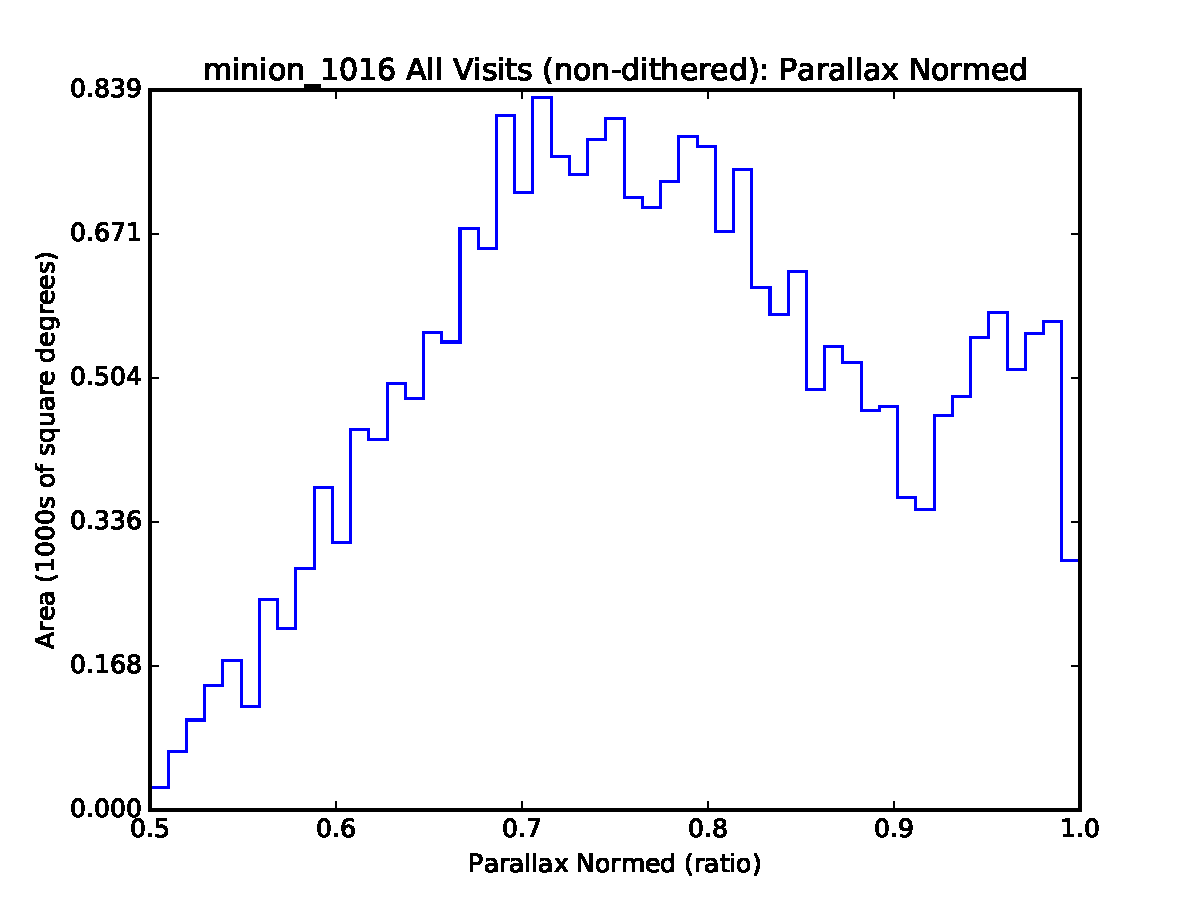
\includegraphics[angle=0,width=0.49\hsize,clip]{figs/cadence/minion_1016_Parallax_Normed_All_Visits_non-dithered_HEAL_Histogram.pdf}
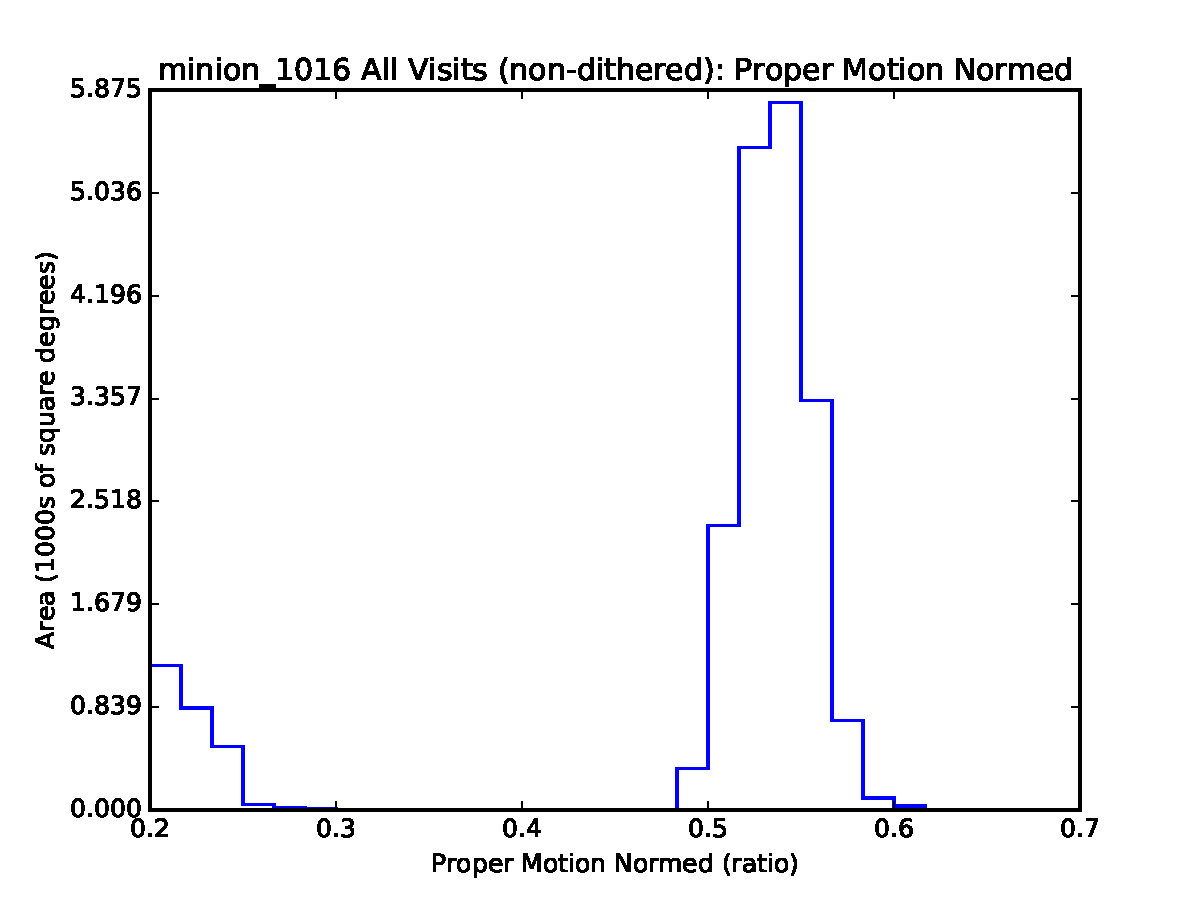
\includegraphics[angle=0,width=0.49\hsize,clip]{figs/cadence/minion_1016_Proper_Motion_Normed_All_Visits_non-dithered_HEAL_Histogram.pdf}
\vskip -0.1in
\caption{The trigonometric parallax errors (left) and proper motion errors (right), normalized
by the values for idealized perfectly optimized cadences (parallax: all the observations are taken
at maximum parallax factor, resulting in a peak at the South Ecliptic pole; proper motion:
a half of all visits are obtained on the first day and the rest on the last day of the survey),
obtained for simulated cadence \opsimdbref{db:baseCadence} are shown in Aitoff projection of equatorial
coordinates.}
\label{fig:parapmenigma}
\end{figure}
%%%%%%%%%%%%%%%%%%%%%%%%%%%%%%%%%


The Baseline Cadence,
\opsimdbref{db:baseCadence}, has the following basic
properties\footnote{For MAF output, see \url{http://ls.st/tny} and
\url{http://ls.st/67x}}:
\begin{enumerate}
\item The total number of visits is 2,447,931, with 85.1\% spent on
the Universal proposal (the main Wide, Fast, Deep (WFD) survey and henceforth
known as the WFD proposal), 6.5\% on the
North Ecliptic Spur proposal, 1.7\% on the Galactic Plane proposal, 2.2\%
on the South Celestial Pole proposal, and 4.5\% on the Deep Drilling
Cosmology proposal (5 fields).\footnote{The community-contributed white papers leading to the
Deep Drilling fields defined in the Baseline Cadence can be found via
\url{https://community.lsst.org/t/deep-drilling-whitepapers/732}.}
\item The median number of visits per night is 816, the range is
88 to 1,104, with 3,026 observing nights. The mean slew time is 6.8
seconds (median: 4.8 sec) and the total exposure time (after 10 yeras) is 73.4 Msec.
The surveying efficiency, or the median total open shutter time (per night)
as a fraction of the observing time (the ratio of the open shutter time to
the sum of the open shutter time, readout time and slew time) is 73\%.
\item
The 25\%-75\% quartiles for the number of filter changes per night are 2
and 6, with the mean of 4.3 The total number of filter changes through the survey is 14,194.
\item In the $r$ band, the median effective seeing for all proposals is 0.93 arcsec (for the more
traditional geometric FWHM, the median is 0.81 arcsec).  We define ``geometric FWHM'' as the actual full-width-at-half-maximum.  The ``Effective FWHM'' is the FWHM of a single Gaussian describing the PSF and is typically $\sim15$\% larger than the geometric FWHM. The median
airmass for all filters and all proposals is 1.23. The median single-visit $5\sigma$ depth for point sources in $r$ band in the WFD area is 24.16 (using the best
current estimate of the fiducial depth at airmass of one, $m_5(r)=24.39$,
defined by the SRD Table 5). The variation of the median airmass for the $r$
band observations with the position on the sky is shown in
\autoref{fig:airmassenigma}.
\item The median single-visit depths for WFD fields are (23.14, 24.47, 24.16,
23.40, 22.23, 21.57) in the $ugrizy$ bands\footnote{Note that these values
depend on externally supplied values for fiducial zenith dark time single-epoch
$5\sigma$ depths; the following values were used in analysis described
here: (23.62, 24.85, 24.39, 23.94, 23.36, 22.45) in the $ugrizy$
bands, respectively. These values are similar, but not identical, to the values
listed in Table 2 from the latest version (v3.1) of the LSST overview
paper: (23.68, 24.89, 24.43, 24.00, 23.45, 22.60). This discrepancy
is due to continuing improvements in the system performance estimates.}.
These values are shallower than
the zenith dark time values for three main reasons: the sky is expected to be
brighter for non-dark time and away from zenith, the sky brightness model
currently implemented in \OpSim has some shortcomings (a new model has been implemented for version 4), and the moon avoidance is not as aggressive
as it could be (many observations are taken very close to the moon avoidance limit of 30 degrees, rather than farther away where the sky is darker). As a result, the median limiting depths above are brighter than typical zenith dark-time images by close
to 1 mag in the $z$ and $y$ bands, and a few tenths of a magnitude in the
$u$, $g$ and $i$ bands.
\item For the 2,293 (overlapping) fields from the WFD area,
the median number of visits in the $ugrizy$ bands is (62, 88, 199, 201, 180,
180), respectively. Not only do these medians exceed the requested
number of visits (design specification from the SRD\footnote{The LSST
Science Requirements Document (SRD) is available as
\url{http://ls.st/lpm-17}}) of (56, 80, 184, 184, 160, 160) in the $ugrizy$
bands, but the minimum number of visits per field over this area does
so, too. This result is quite encouraging given that
only 85\% of observing time was spent on the WFD Cadence proposal.
\item The median coadded $5\sigma$ depth
for point sources in the $ugrizy$ bands is (25.4, 27.0, 27.1, 26.4,
25.2, 24.4), respectively, for the WFD area. The distribution
of coadded depth across the sky is fairly uniform, as illustrated in \autoref{fig:coaddm5enigma}.
\item For the 2,293 fields from the WFD area, the median
geometric FWHM for seeing is 0.78 arcsec in the $r$ band and 0.77 arcsec
in the $i$ band. The median airmass in the $urz$ bands is 1.25, 1.20 and 1.26
(the maximum allowed airmass for the WFD area was set to
1.5).  The median sky brightness in the $ury$ bands is 22.0 mag/arcsec$^2$,
21.1 mag/arcsec$^2$, and 17.3 mag/arcsec$^2$, respectively (for comparison, the
assumed dark sky brightness at zenith in the $ury$ bands is 23.0, 21.2 and 18.6
mag/arcsec$^2$).  The current model sky brightness in the $y$ band is biased
very high because most $y$ band (and many $z$ band) observations are taken in twilight where \OpSim currently uses a very simple (and bright) sky model.
\item Restricted to the WFD fields, a unique area of
18,000 square degrees received at least 888 visits per field (summed over bands;
the SRD design value is 825).
\item The median trigonometric parallax and proper motion errors are
0.62 mas and 0.17 mas/yr, respectively, for bright sources (limited by
assumed systematic errors in relative astrometry of 10 mas), and 7.9
mas and 2.3 mas/yr for points sources with $r=24$ (assuming flat
spectral energy distribution), over the WFD fields. The
variation of parallax and proper motion errors across the sky is
visualized in \autoref{fig:parapmenigma}.
\end{enumerate}





For comparison, the old Baseline Cadence, \texttt{opsim3.61}
(obtained with an older version of the \OpSim code), delivered 2,651,588 visits, or 8.3\%
more than \opsimdbref{db:baseCadence}  (this is due to known effects and
changes in the code,  such as more pre-scheduled down time in the new
version). Perhaps the most important (and undesired!) difference
between the two simulations is that the Baseline Cadence
spent 6.5\% of the observing time on the North Ecliptic Spur proposal (vs.
4\% spent on the corresponding Universal North proposal in
\texttt{opsim3.61}), and less than 90\% of time on the WFD proposal.

Analysis of the hour angle distribution, shown in
\autoref{fig:HAenigma} and \autoref{fig:AltAzenigma}, reveals a strong
bias towards observations west from the meridian for the main survey.
This pattern is being investigated: it may be
caused by specific features of the cost function implemented in the
\OpSim code. Removing the bias has the potential to increase the survey depth by around $\sim10\%$ (the survey would reach it's current limiting depth in 9 years rather than 10).



%%%%%%%%%%%%%%%%%%%%%%%%%%%%%%%%%
\begin{figure}[t!]
\vskip -0.0in
\includegraphics[angle=0,width=0.49\hsize,clip]{figs/cadence/minion_1016_Hour_Angle_Histogram_u_g_r_i_z_y_band_all_props_ONED_ComboBinnedData.pdf}
\includegraphics[angle=0,width=0.49\hsize,clip]{figs/cadence/minion_1016_Mean_HA_r_band_all_props_OPSI_SkyMap.pdf}
\vskip -0.1in
\caption{Histograms in the left panel show the distribution of hour angles (HA) in
6 bands for all proposals from simulated cadence \opsimdbref{db:baseCadence} (the distributions are
similar for WFD fields considered alone). Note the bias towards observations west from
the meridian. The right panel shows the distribution across the sky of the mean HA for
all observations in the $r$ band. }
\label{fig:HAenigma}
\end{figure}
%%%%%%%%%%%%%%%%%%%%%%%%%%%%%%%%%

%%%%%%%%%%%%%%%%%%%%%%%%%%%%%%%%%
\begin{figure}[t!]
\vskip -0.0in
\includegraphics[angle=0,width=0.49\hsize,clip]{figs/cadence/minion_1016_Nvisits_as_function_of_Alt_Az_all_observations_HEAL_SkyMap.pdf}
\includegraphics[angle=0,width=0.49\hsize,clip]{figs/cadence/minion_1016_Nvisits_as_function_of_Alt_Az_r_Universal-18-0824B_HEAL_SkyMap.pdf}
\vskip -0.1in
\caption{The color-coded map in the left panel shows the visit count from the
Baseline Cadence simulation \opsimdbref{db:baseCadence} in the equal-area Lambert projection of the
horizontal coordinate system (altitude-azimuth), with north on top and west towards the
right, for all six bands and proposals (Wide, Fast, Deep, Galactic Plane, Deep Drilling
fields, North Ecliptic Spur, and South Celestial Pole region). The WFD Cadence was
limited to airmass below 1.5, while other proposals sampled higher airmass, too (see the
histogram in \autoref{fig:airmassenigma}).  Note the strong propensity of fields
for westward observations (the median airmass is about 1.2). The right panel is analogous,
but only shows the $r$ band visits for WFD fields.}
\label{fig:AltAzenigma}
\end{figure}
%%%%%%%%%%%%%%%%%%%%%%%%%%%%%%%%%







%%%%%%%%%%%%%%%%%%%%%%%%%%%%%%%%%
\begin{figure}[th!]
\vskip -0.0in
\includegraphics[angle=0,width=0.49\hsize,clip]{figs/cadence/minion_1016_Position_Angle_Histogram_u_g_r_i_z_y_band_WFD_ONED_ComboBinnedData.pdf}
\includegraphics[angle=0,width=0.49\hsize,clip]{figs/cadence/minion_1016_RmsAngle_rotSkyPos_r_band_WFD_OPSI_SkyMap.pdf}
\vskip -0.1in
\caption{The left panel shows the position angle distribution (in radians)  in each band for the
main survey fields in \opsimdbref{db:baseCadence}. The position angle is the angle between
``up'' in the image and North on the sky. The variation of the root-mean-square scatter of the
$r$ band distribution across the sky is shown in the right panel.}
\label{fig:rotator}
\end{figure}
%%%%%%%%%%%%%%%%%%%%%%%%%%%%%%%%%

Another potentially undesirable feature, seen in practically all
simulations analyzed here, is that up to about a quarter of visits in
the main survey area represents the third, the fourth and sometimes
even the fifth visit to a field in the same night. For a large number
of time-domain programs, these visits could be used instead to
decrease the field inter-night revisit time. For more details, see
\autoref{sec:solarsystem:discovery}. The position angle distributions for this simulation
are shown in \autoref{fig:rotator}.


\subsubsection{Time-domain Analysis}

\autoref{fig:enigmaGapAll} shows the median revisit time distribution
when all bands are considered, and \autoref{fig:enigmaGapr} shows the
median revisit time distribution in the band.  On average, fields in
the main survey get revisited about every 3 days using all filters,
and every 15 days when using only $r$ band visits (30 days when using
only $u$ band visits is the longest median revisit time).
\autoref{fig:enigmaMAXGapAll} shows the maximum inter-night gap, which
on average is about 5-6 months.

The temporal sampling for this simulation is sufficient to enable a
large recovery fraction for SNe. \autoref{fig:enigmaEarlySNe} shows
that a large fraction of LSST SNe will be detected before their
maximum brightness. Metrics for transient objects
are discussed in \autoref{chp:transients}, and the supernova section (\ref{sec:supernovae}) of \autoref{chp:cosmo}.
Intra-night revisit time distribution is discussed in more detail in
\autoref{sec:solarsystem:discovery}. The analysis of asteroid completeness is
discussed in \autoref{sec:solarsystem:discovery}.



%%%%%%%%%%%%%%%%%%%%%%%%%%%%%%%%%
\begin{figure}[t!]
\vskip -0.0in
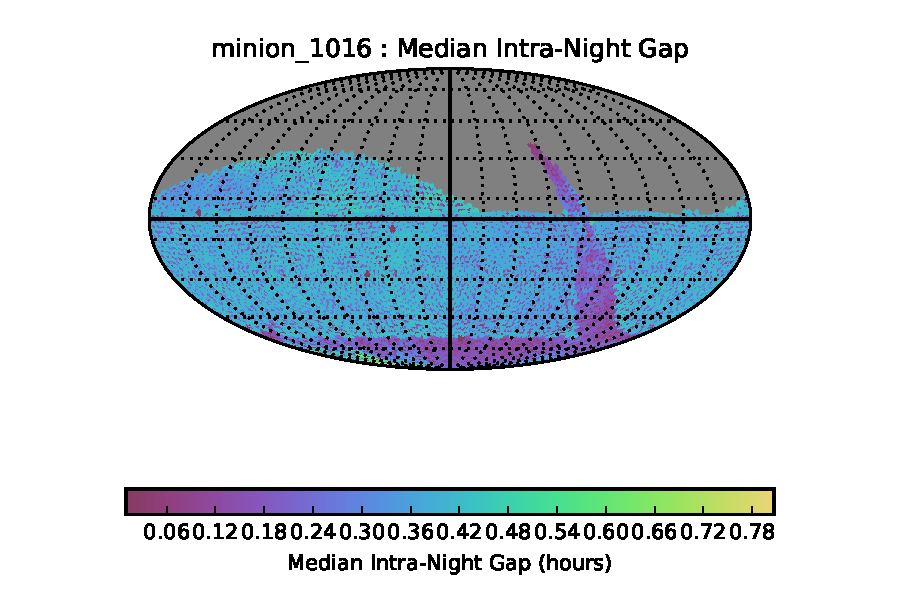
\includegraphics[angle=0,width=0.49\hsize,clip]{figs/cadence/minion_1016_Median_Intra-Night_Gap_HEAL_SkyMap.pdf}
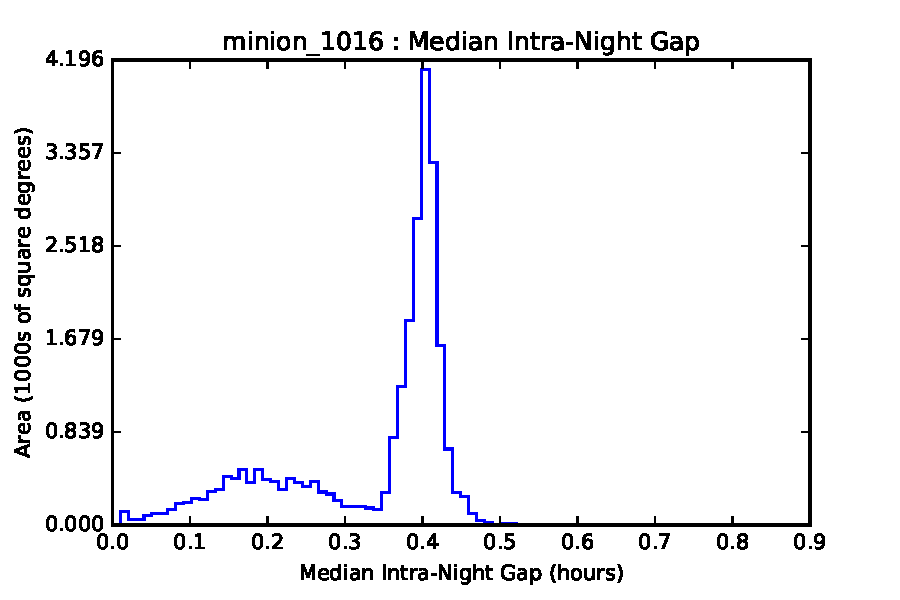
\includegraphics[angle=0,width=0.49\hsize,clip]{figs/cadence/minion_1016_Median_Intra-Night_Gap_HEAL_Histogram.pdf}
\vskip -0.1in
\caption{The median intra-night gap (or revisit time) is shown in Aitoff projection
for all proposals and all filters for the Baseline Cadence \opsimdbref{db:baseCadence}.
On average, when a field is observed multiple times in a night there is a 25 minute gap between the observations.}
\label{fig:enigmaInterGapAll}
\end{figure}
%%%%%%%%%%%%%%%%%%%%%%%%%%%%%%%%%


%%%%%%%%%%%%%%%%%%%%%%%%%%%%%%%%%
\begin{figure}[t!]
\vskip -0.0in
\includegraphics[angle=0,width=0.49\hsize,clip]{figs/cadence/minion_1016_Median_Inter-Night_Gap_HEAL_SkyMap.pdf}
\includegraphics[angle=0,width=0.49\hsize,clip]{figs/cadence/minion_1016_Median_Inter-Night_Gap_HEAL_Histogram.pdf}
\vskip -0.1in
\caption{The median inter-night gap (or revisit time) is shown in Aitoff projection
for all proposals and all filters for the Baseline Cadence \opsimdbref{db:baseCadence}.
On average, fields in the main survey get revisited about every 3 days.}
\label{fig:enigmaGapAll}
\end{figure}
%%%%%%%%%%%%%%%%%%%%%%%%%%%%%%%%%

%%%%%%%%%%%%%%%%%%%%%%%%%%%%%%%%%
\begin{figure}[h!]
\vskip -0.0in
\includegraphics[angle=0,width=0.49\hsize,clip]{figs/cadence/minion_1016_Median_Inter-Night_Gap_r_HEAL_SkyMap.pdf}
\includegraphics[angle=0,width=0.49\hsize,clip]{figs/cadence/minion_1016_Median_Inter-Night_Gap_r_HEAL_Histogram.pdf}
\vskip -0.1in
\caption{The median inter-night gap for $r$ band visits is shown in Aitoff projection
for all proposals for the Baseline Cadence \opsimdbref{db:baseCadence}.
On average, fields in the main survey get revisited in the $r$ band about every two weeks.}
\label{fig:enigmaGapr}
\end{figure}
%%%%%%%%%%%%%%%%%%%%%%%%%%%%%%%%%

%%%%%%%%%%%%%%%%%%%%%%%%%%%%%%%%%
\begin{figure}[t!]
\vskip -0.0in
\includegraphics[angle=0,width=0.49\hsize,clip]{figs/cadence/minion_1016_Max_Inter-Night_Gap_HEAL_SkyMap.pdf}
\includegraphics[angle=0,width=0.49\hsize,clip]{figs/cadence/minion_1016_Max_Inter-Night_Gap_HEAL_Histogram.pdf}
\vskip -0.1in
\caption{The maximum inter-night gap (or revisit time) is shown in Aitoff projection
for all proposals and all filters for the Baseline Cadence \opsimdbref{db:baseCadence}.}
\label{fig:enigmaMAXGapAll}
\end{figure}
%%%%%%%%%%%%%%%%%%%%%%%%%%%%%%%%%



%%%%%%%%%%%%%%%%%%%%%%%%%%%%%%%%%
\begin{figure}[h!]
\vskip -0.0in
\includegraphics[angle=0,width=0.49\hsize,clip]{figs/cadence/minion_1016_SNAlert_HEAL_SkyMap.pdf}
\includegraphics[angle=0,width=0.49\hsize,clip]{figs/cadence/minion_1016_SNAlert_HEAL_Histogram.pdf}
\vskip -0.1in

\caption{The fraction of simulated Type Ia SNe at a redshift of 0.5 detected
pre-peak in any filter for the Baseline Cadence \opsimdbref{db:baseCadence}. About
40\% of all such SNe from the main survey will be detected before their
maximum brightness.}
\label{fig:enigmaEarlySNe}
\end{figure}
%%%%%%%%%%%%%%%%%%%%%%%%%%%%%%%%%



\subsubsection{Special Proposals}

Regarding the special proposals, here we only provide the basic
performance parameters. With the exception of the Deep Drilling
proposal, these proposals are essentially strawman placeholders. The
North Ecliptic Spur proposal (6.4\% of the observing time) obtained  300 visits per field, summed over $griz$ bands. These
fields are placed along the northern part of the Ecliptic. The
Galactic Plane proposal (1.7\%) obtained 30 visits per band in all six
bands, across the region extending in Galactic latitude 10 degrees
from the Galactic center, with the boundary approaching the Galactic
equator linearly with longitude, and the zone ending at $l=90$ deg.
and at $l=270$ deg. The South Celestial Pole proposal (2.1\%) obtained
30 visits per band in all six bands, for fields centers with Dec $<
-62.5$ deg. The Deep Drilling proposal (4.5\%) included 5
fields, with each obtaining several thousand visits per band as required for various cosmology investigations. The
coadded $5\sigma$ depths for these fields are much fainter than for
the main survey: the median values are (27.8, 28.4, 28.6, 28.0, 27.6,
26.1) in the $ugrizy$ bands, respectively.


\vskip 0.2in
{\bf Conclusions:}

The Baseline Cadence, \opsimdbref{db:baseCadence}, appears to
be an adequate replacement for the old Baseline Cadence
(\texttt{opsim3.61}). Based on this analysis, there are no
major problems with its performance. While there are patterns which
are not fully understood (most notably the observing bias towards
west),  or undesired (unnecessary revisits of the same field in the
same night), \opsimdbref{db:baseCadence} is used as a benchmark cadence,
and referred to as the ``Baseline Cadence'', in the rest of this
document. This simulation was proposed by the Project Science Team
and adopted as the new Baseline Cadence by the LSST Change Control Board in August 2016.

An important feature of \opsimdbref{db:baseCadence} simulation is that
the mean slew time of 6.8 sec (which includes filter change time) is
very close to the minimum possible slew time of about 4.5 sec. The
implication is that the surveying efficiency, assuming 30 sec exposure
time per visit, can be increased by at most about 6\% (that is, the
total open-shutter time is within about 6\% from its possible maximum,
given everything else unchanged).  Nevertheless, there are other
survey aspects, including sky coverage and temporal sampling
functions, that can be further optimized, as discussed in
\autoref{sec:cadexp:alternatives} below.

{\bf The main remaining known problems} with \opsimdbref{db:baseCadence} simulation include
\begin{itemize}
\item A strong bias towards observations west from the meridian for
  the main survey, see \autoref{fig:AltAzenigma}.  This bias
  significantly degrades the survey seeing and depth.
\item Several proposals complete after only 3-4 years, resulting in
  regions of sky where the proper motions are poorly constrained due
  to the short observing baseline.  See \autoref{fig:parapmenigma2}.
\item The sky brightness model has systematic errors, particularly in twilight time,
  resulting in estimates of limit depths ($m_5$ for single
  visits and coadded depths) that are too shallow by about 0.3 mag in
  the $u$ band, and 0.5-1.0 mag in the $z$ and $y$ bands.
\item The moon avoidance angle of 30 deg. allows too many $z$ band
  observations with elevated sky brightness due to moonshine,
  resulting in about 0.2-0.3 mag shallower depth.
\item There are too many unrequested and unnecessary revisits of the
  same field in the same night (that is, more than two visits to the
  same field in the same night).
\end{itemize}
Most of these issues are expected to be resolved by \OpSim version 4.

\navigationbar
% --------------------------------------------------------------------








% --------------------------------------------------------------------

\section{Some Simulated Alternative Observing Strategies}
\def\secname{cadexp:alternatives}\label{sec:\secname}

We now describe some alternatives to the Baseline Cadence that were
explored. These \OpSim databases are all available for further testing
with science-based MAF metrics.

% - - - - - - - - - - - - - - - - - - - - - - - - - - - - - - - - - -

%%%%%%%%%%%%%%%%%%%%%%%%%%%%%%%
\opsimdb[db:opstwo]{minion\_1012}{Only Wide, Fast, Deep Cadence, with pairs of visits.}
%%%%%%%%%%%%%%%%%%%%%%%%%%%%%%%

{\bf Motivation and description:} Formally, $\sim$85\% of observing
time is allocated to the main WFD Cadence program. The
remaining observing time is allocated to other programs, such as
``Deep Drilling'' programs (see Section 3.4 and Tables 22-26  in the
SRD). With this simulation, we wished to find out what would be the
effect of ignoring special programs and spending all of the observing
time on the main WFD Cadence program. \\

{\bf Expectations:} About 2.08 million visits (85\% of 2.44 million
visits) from the Baseline Cadence (\opsimdbref{db:baseCadence}) were allocated
to WFD Cadence. With \opsimdbref{db:opstwo} we expect that all of these 2.44 million visits
will be allocated to WFD Cadence. \\

{\bf Analysis Results:} This simulated cadence is named \opsimdbref{db:opstwo}.
Compared to the Baseline Cadence \opsimdbref{db:baseCadence}:
\begin{enumerate}
\item The total number of visits is close to the expected value: 2.42
  million.  The minimum number of visits per field for the 2,293 WFD
  fields in the Baseline Cadence is 965 for this simulation, compared to
  888 for the Baseline Cadence.
\item The median number of visits per night and the mean slew time are
  essentially the same as for the Baseline Cadence (807 vs. 816 and 7.2
  sec vs. 6.8 sec).
\item The median seeing, sky brightness and airmass in the $r$ and $i$ bands are
      essentially the same as for WFD fields in the Baseline Cadence.
\item The median trigonometric parallax and proper motion errors are
  improved by about 8\%, with improvements commensurate with the
  increase in the number of visits and the elimination of regions
  which are not observed for a full 10 years.
\item This simulation also shows observing bias towards west (that is,
  additional special programs in \opsimdbref{db:baseCadence} are not
  responsible for this bias).
\end{enumerate}


{\bf Conclusions:} \opsimdbref{db:opstwo}, using only the WFD Cadence
proposal, delivered 99.2\% of the number of visits obtained by the
Baseline Cadence. Therefore, {\it the ``filler'' aspect of other
proposals does not have a major impact on the surveying efficiency}.
The minimum number of visits per field for the 2,293 WFD fields in the
Baseline Cadence is 886 (the SRD design value is 825 and the stretch
goal value is 1000). Although the sky coverage of these 2293 fields is
about 18,000 sq.deg., that number of fields could cover 22,000 sq.deg if there was no field overlap. With
proper dithering (see \eg \autoref{sec:lss}), the effective number of visits could be increased to
$886\times22/18 = 1083$ (or the WFD area increased from 18,000 sq.deg.; see
analysis of \opsimdbref{db:opstwoPS} below). This increase is an improvement of 31\%
relative to the SRD design specification of 825 visits over 18,000
sq.deg. However, note again that there are no other programs in this
simulation (i.e., if other programs were allocated 10\% of the
observing time, the implied overall ``over-performance'' in the number
of  visits would be about 20\%).

% - - - - - - - - - - - - - - - - - - - - - - - - - - - - - - - - - -

%%%%%%%%%%%%%%%%%%%%%%%%%%%%%%%%%
\opsimdb[db:opstwoPS]{minion\_1020}{A Pan-STARRS-like observing strategy.}
%%%%%%%%%%%%%%%%%%%%%%%%%%%%%%%%%

{\bf Motivation and description:} ``Pan-STARRS-like cadence" attempts to apply a
uniform cadence strategy throughout the maximum size survey region, which is about 27,400~deg$^2$. This is similar to the Pan-
STARRS' 3PI survey which also tries to maximize sky area. The maximum acceptable
airmass is kept at its default value of 1.5; this excludes fields with Dec~$<-78$~deg and Dec~$> +18$~deg. The \opsimdbref{db:opstwoPS} simulations utilizes a maximum Dec of $+15$~deg, uniform cadence and no
other proposal, and requires pairs of visits as in the Baseline Cadence. \\

{\bf Expectations:} The total number of visits should be roughly the
same as in the Baseline Cadence, but spread over a 42\% larger sky area
(3,255 fields instead of 2,293), with fewer visits per field. \\

{\bf Analysis Results:}  This simulated cadence is named \opsimdbref{db:opstwoPS}.
Compared to the Baseline Cadence \opsimdbref{db:baseCadence}:
\begin{enumerate}
\item The total number of visits is 2.42 million, and essentially identical to the
number of visits in the Baseline cadence.
\item
The mean number of visits per field is 740, which is 81\% of the number of visits %minion_1016 median 912 visits per feild WFD
for WFD fields obtained by the Baseline Cadence (but here the sky area is 42\% larger). We note that this is below the number required by the SRD.
\item The median number of visits per night and the mean slew time are
  essentially the same as for the Baseline Cadence.
\item The median seeing, sky brightness and airmass in the $r$ and $i$
  bands for WFD fields are essentially the same as in the Baseline
  Cadence.
\item The median trigonometric parallax and proper motion errors show
  uniform behavior over the entire enlarged area (see
  \autoref{fig:parapmenigma2}), with the values similar to those
  obtained for the Baseline Cadence.
\item This simulation also shows observing bias towards west.
\end{enumerate}

Due to increased sky area, which samples regions that can never
achieve low airmass, the median coadded depth is about 0.15 mag
shallower for this simulation than for the Baseline Cadence. As a result,
the counts of galaxies per unit area down to a fixed SNR would
decrease by about 15-20\%. At the same time, the area outside the
Galactic plane is increased by about 30\%, and thus the total number
of galaxies would be increased by about 10\%, compared to WFD fields
in the Baseline Cadence. However, the increased median airmass also
results in larger seeing, especially for the borderline regions, as
illustrated in \autoref{fig:PS-seeing}. The increased median seeing
would decrease the number of galaxies effectively resolved for weak
lensing by about 3-5\%. In addition, the additional area has somewhat
larger extinction due to interstellar dust which further decreases the
galaxy counts (this impact of dust extinction on galaxy counts is not
yet implemented in MAF). As a result of these effects, the two
strategies result in similar weak lensing galaxy samples.

{\bf Conclusions:} When only the WFD Cadence proposal is
employed, the survey area could be increased by about 40\%, while
still delivering the mean number of fields at the level of 81\% of
that in the Baseline Cadence (or 90\% of the SRD design value of 825).
Hence, simulations \opsimdbref{db:opstwoPS} and \opsimdbref{db:opstwo}
demonstrate that this hypothetical ``survey reserve'', relative to the WFD
Cadence design specifications from the SRD, can be used to i) increase
the number of visits per field over the WFD area, or ii) increase the
surveyed area while keeping the number of visits per field
statistically unchanged, or iii) increase both area and the number of
visits, and/or iv) execute additional programs (the current baseline).
Of course, it must be remembered that this ``survey reserve'' is derived
using design system characteristics and thus unproven at the time of
writing.


%%%%%%%%%%%%%%%%%%%%%%%%%%%%%%%%%
\begin{figure}[t!]
\vskip -0.03in
\includegraphics[angle=0,width=0.49\hsize:,clip]{figs/cadence/minion_1020_Parallax_Normed_All_Visits_non-dithered_HEAL_SkyMap.pdf}
\includegraphics[angle=0,width=0.49\hsize:,clip]{figs/cadence/minion_1020_Proper_Motion_Normed_All_Visits_non-dithered_HEAL_SkyMap.pdf}
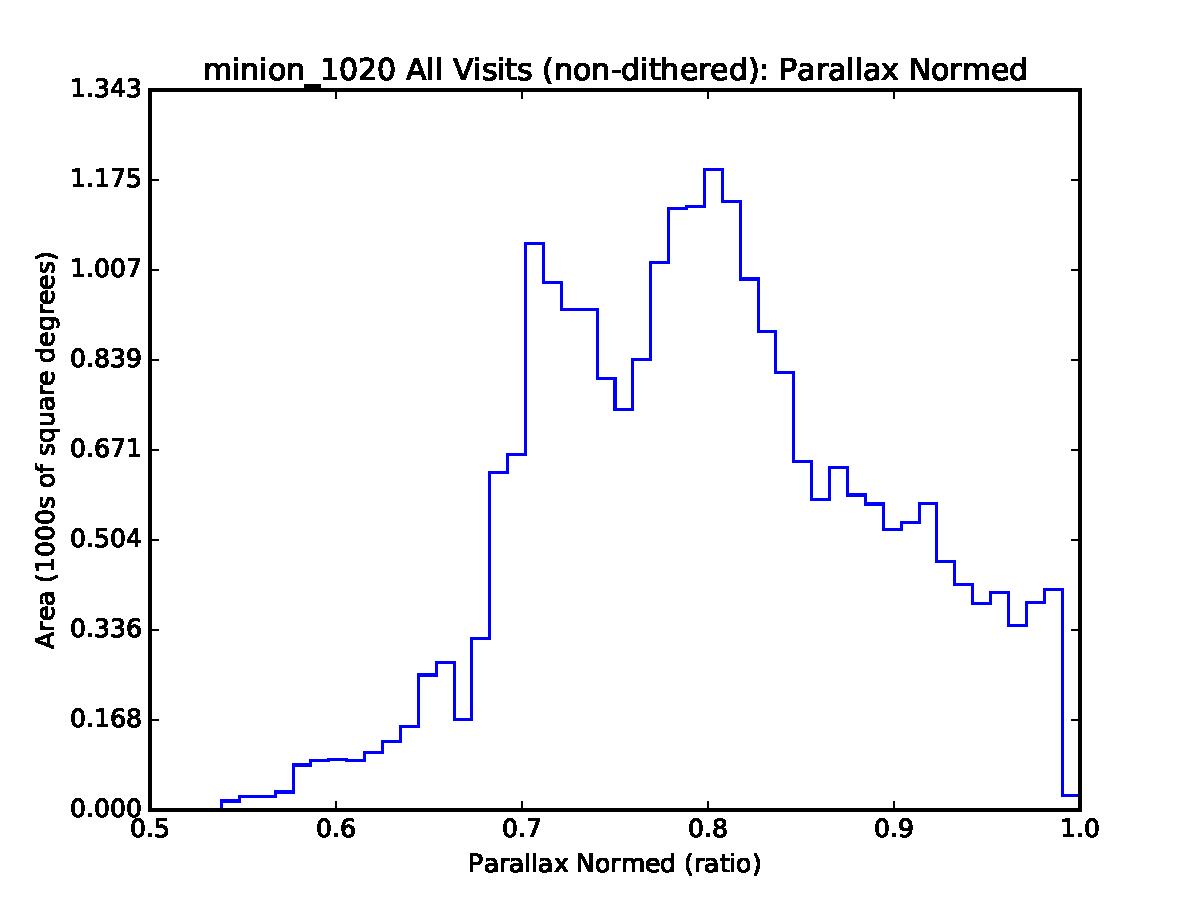
\includegraphics[angle=0,width=0.49\hsize:,clip]{figs/cadence/minion_1020_Parallax_Normed_All_Visits_non-dithered_HEAL_Histogram.pdf}
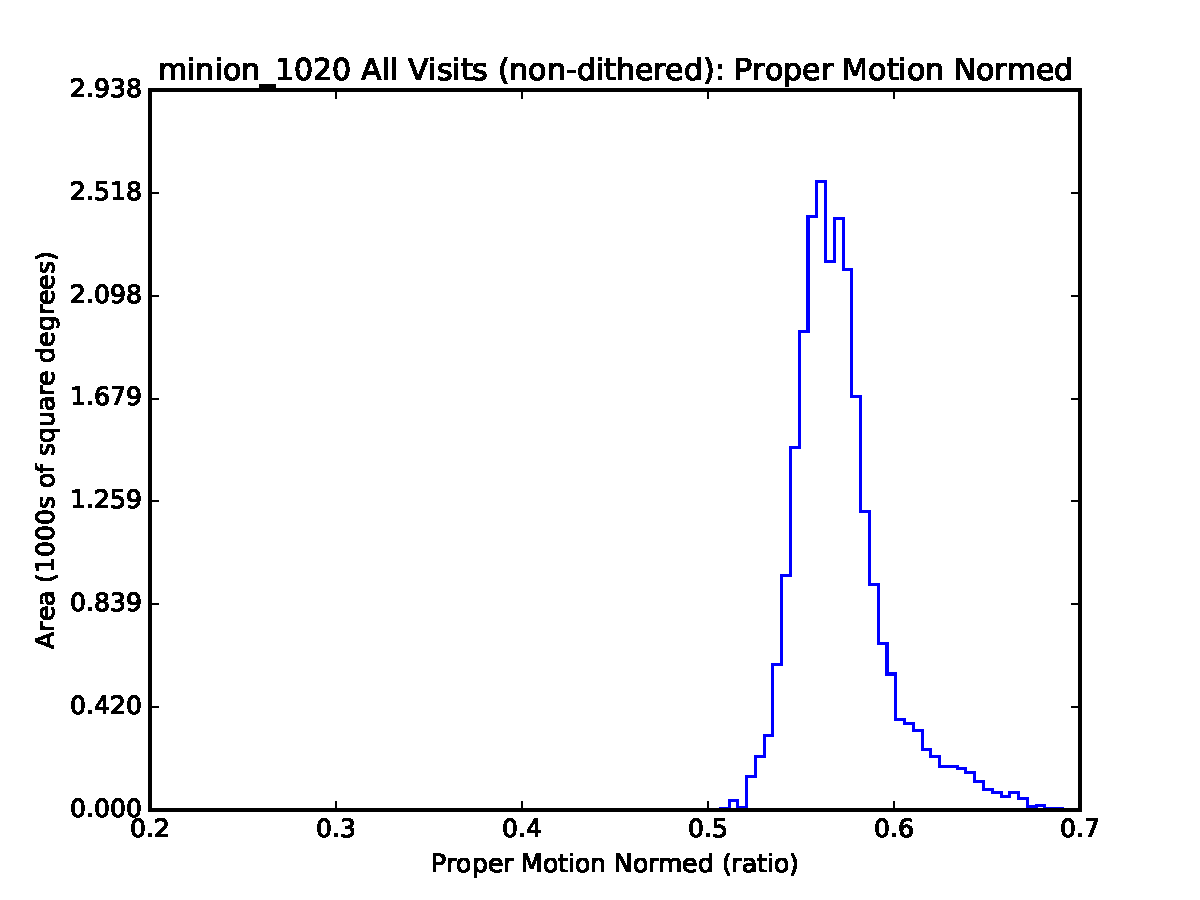
\includegraphics[angle=0,width=0.49\hsize:,clip]{figs/cadence/minion_1020_Proper_Motion_Normed_All_Visits_non-dithered_HEAL_Histogram.pdf}
\vskip -0.2in
\caption{The trigonometric parallax errors (left) and proper motion errors (right) for simulated cadence
minion\_1020 (``Pan-STARRS-like'' Cadence), normalized by the values for idealized perfectly optimized
cadence, are shown in Aitoff projection of equatorial coordinates (compare to \autoref{fig:parapmenigma}).}
\label{fig:parapmenigma2}
\end{figure}
%%%%%%%%%%%%%%%%%%%%%%%%%%%%%%%%%

%%%%%%%%%%%%%%%%%%%%%%%%%%%%%%%%%
\begin{figure}[t!]
\vskip -0.03in
\includegraphics[angle=0,width=0.49\hsize:,clip]{figs/cadence/minion_1020_Median_FWHMeff_r_band_all_props_OPSI_SkyMap.pdf}
\includegraphics[angle=0,width=0.49\hsize:,clip]{figs/cadence/minion_1020_Median_FWHMeff_r_band_all_props_OPSI_Histogram.pdf}
\vskip -0.2in
\caption{The median seeing in $r$ filter, for simulated cadence minion\_1020 (``Pan-STARRS-like'' Cadence),
normalized by expected value (0.83$^{\prime\prime}$). Note that fields with the most positive and most negative
declination have on average larger values. For comparison, the median normalized seeing for WFD fields
in the Baseline Cadence is 1.08, with a negligible fraction of fields with values above 1.18.}
\label{fig:PS-seeing}
\end{figure}
%%%%%%%%%%%%%%%%%%%%%%%%%%%%%%%%%


% - - - - - - - - - - - - - - - - - - - - - - - - - - - - - - - - - -

%%%%%%%%%%%%%%%%%%%%%%%%%%%%%%%%%%%%%%%%%%%
\opsimdb[db:UConlyNoVisitPairs]{minion\_1013}{Only Wide, Fast, Deep Cadence, no visit pairs.}
%%%%%%%%%%%%%%%%%%%%%%%%%%%%%%%%%%%%%%%%%%%

{\bf Motivation and description:} The main goal of this simulation was
to assess the impact of the requirement for visit pairs on the survey
efficiency (the Baseline Cadence requests two visits per night to the same
field, separated in time by about an hour, and driven by asteroid
orbit determination). It is plausible that the removal of this
requirement could result in a more efficient survey. In order to allow
as simple analysis as possible, only the WFD Cadence proposal is
requested. Hence, this simulation should be directly compared to
simulation \opsimdbref{db:opstwo}. \\

{\bf Expectations:} If the requirement for visit pairs decreases
surveying efficiency, then this simulation should deliver more than
the 2.42~million visits delivered by \opsimdbref{db:opstwo}. \\

{\bf Analysis Results:} This simulated cadence is named \opsimdbref{db:UConlyNoVisitPairs}. Compared
to \opsimdbref{db:opstwo}:
\begin{enumerate}
\item The total number of visits is 2.42 million, identical to \opsimdbref{db:opstwo}.
\item The median slew time, and the median coadded depth and seeing in the $r$ band
are essentially identical, too.
\item The median airmass in the $r$ band of 1.25 is a bit higher than 1.18 obtained
for \opsimdbref{db:opstwo}.
\item The median fraction of revisits faster than 30 minutes of 0.32 is smaller than 0.38
for \opsimdbref{db:opstwo}, and is consistent with the absence of pair contributions (that is,
such revisits are due to field edge overlaps, and unintentional revisits, in case of \opsimdbref{db:UConlyNoVisitPairs}).
\end{enumerate}

{\bf Conclusions:} The comparison of this simulation and
\opsimdbref{db:opstwo} shows that requiring pairs of visits (in a
given observing night) does not result in an appreciable loss of
surveying efficiency. Indeed, pairs of visits result in a better
short-timescale coverage that would enhance many types of time-domain
science (and, of course, it's crucial for asteroid science).


% - - - - - - - - - - - - - - - - - - - - - - - - - - - - - - - - - -

%%%%%%%%%%%%%%%%%%%%%%%%%%%%%%%%%%%%%%%%%%%
\opsimdb[db:NoVisitPairs]{kraken\_1043}{Baseline Cadence, but with no visit pairs.}
%%%%%%%%%%%%%%%%%%%%%%%%%%%%%%%%%%%%%%%%%%%

{\bf Motivation and description:} The main goal of this simulation was
to assess the impact of the requirement for visit pairs on the survey
efficiency. Instead of the idealized case above which compared only
the WFD Cadence proposal fields, in this more realistic case
{\it all proposals from the Baseline Cadence are executed}. Hence, this
simulation should be compared to the Baseline Cadence
(\opsimdbref{db:baseCadence}). \\

{\bf Expectations:} A slight, or no, increase in surveying efficiency
and thus the total number of visits is expected when compared to the
Baseline Cadence. \\

{\bf Analysis Results:}  This simulated cadence is named
\opsimdbref{db:NoVisitPairs}. Compared to \opsimdbref{db:baseCadence},
\begin{enumerate}
\item The total number of visits is 2.51 million, or 2.4\% more than
in the Baseline Cadence.
\item The mean slew time is 5.8 sec, or 15\% shorter than for the Baseline
Cadence. This decrease in the mean slew time implies an efficiency
increase of 2.8\% and explains the actual 2.4\% improvement implied by
the total number of visits.  Note that this simulation has the
shortest mean slew time of all simulations investigated here (the
nominal shortest slew and settle time is about 4.5 sec).
\item The median airmass in the $r$ band is slightly larger for this
simulation than for the Baseline Cadence: 1.29 vs. 1.22.
\end{enumerate}


{\bf Conclusions:}
Unlike the comparison of \opsimdbref{db:UConlyNoVisitPairs} and
\opsimdbref{db:opstwo}, here the removal of visit pair requirement
results in a 15\% shorter mean slew time and consequently in 2.4\%
more visits.

% % - - - - - - - - - - - - - - - - - - - - - - - - - - - - - - - - - -
%
% %%%%%%%%%%%%%%%%%%%%%%%%%%%%%%%%%%%%%%%%%%%
\opsimdb[db:NEOswithVisitTriplets]{enigma\_1281}{NEO test: triplets of visits.}
\opsimdb[db:NEOwithVisitQuads]{enigma\_1282}{NEO test: quads of
  visits.}
% %%%%%%%%%%%%%%%%%%%%%%%%%%%%%%%%%%%%%%%%%%%

{\bf Motivation and description:} Many science programs can benefit
from having more than a pair of visits in a night; in particular,
Solar System science may critically depend on having more than just a
pair, depending on the performance of the Moving Object Pipeline
Software (MOPS). These two simulations were run to investigate the
effects of requiring more than just a pair of visits in each
night. The first, \opsimdbref{db:NEOswithVisitTriplets}, requests
sets of three visits (triplets) in each night. The second,
\opsimdbref{db:NEOwithVisitQuads}, requests sets of four visits (quads)
in each night. There is no constraint on the filter chosen for these
sets of visits -- it may be changed or it may remain the same. These
simulations should be compared to the Baseline Cadence,
\opsimdbref{db:baseCadence}, and to the \opsimdbref{db:NoVisitPairs},
which all keep the special surveys, but simply vary the sequences
requested in the WFD Cadence. \\

{\bf Expectations:} The general expectations are that science cases
which require many visits on timescales of a few hours will benefit
with these runs, while science cases which prefer visits to be spaced
more widely over time will see negative impacts.\\

{\bf Analysis Results:}
First, we emphasize that ``requested'' is not the same as
``delivered'': even the ``no pairs''
simulation \opsimdbref{db:NoVisitPairs} ends
up having multiple visits in a given night to the same fields, and
when multiple visits per night are requested, not all fields get to
have completed sequences. The statistics of how many fields are
combined into sequences of a given number of visits is shown in
\autoref{fig:NvisitStats}.  As evident, the highest peak is at the
requested number of visits in a sequence, but not all visits are
incorporated into requested sequences: some are in both shorter and
longer sequences. The ``no pairs'' simulation includes
multiple visits to some fields, because the current
version of the algorithm is not told not to do so. As illustrated in
\autoref{fig:intranightgapCompare}, such revisits typically happen
within 10 minutes from the first visit. This (unintended) behavior
implies that the naive expectation above is probably incorrect, or at
least softened.

The median inter-night revisit rate is affected by requesting more
visits within single night, as expected -- there are only so many
visits available, and if more occur in a particular night, it is
likely (without some kind of rolling cadence) that the result is
longer intervals between subsequent nights. This is demonstrated in
\autoref{fig:internightgapCompare}, where it can be seen that the
inter-night revisit rate increases by about 30\% from 3 nights to 4
nights if we go from pairs to triplets (or quads).

Details of the impacts on Solar System science is
left to \autoref{chp:solarsystem}, in particular the impact on
completeness is evaluated in \autoref{sec:solarsystem:discovery}.

The impact of requesting sequences with 3 or 4 visits to the same
field on other science programs is not yet analyzed in detail.  The
impact on static science should be minimal, except perhaps for a bit
worse behavior of various systematic errors (because fewer nights,
with their observing conditions, are sampled).

%%%%%%%%%%%%%%%%%%%%%%%%%%%
\begin{figure}[t!]
\vskip -0.03in
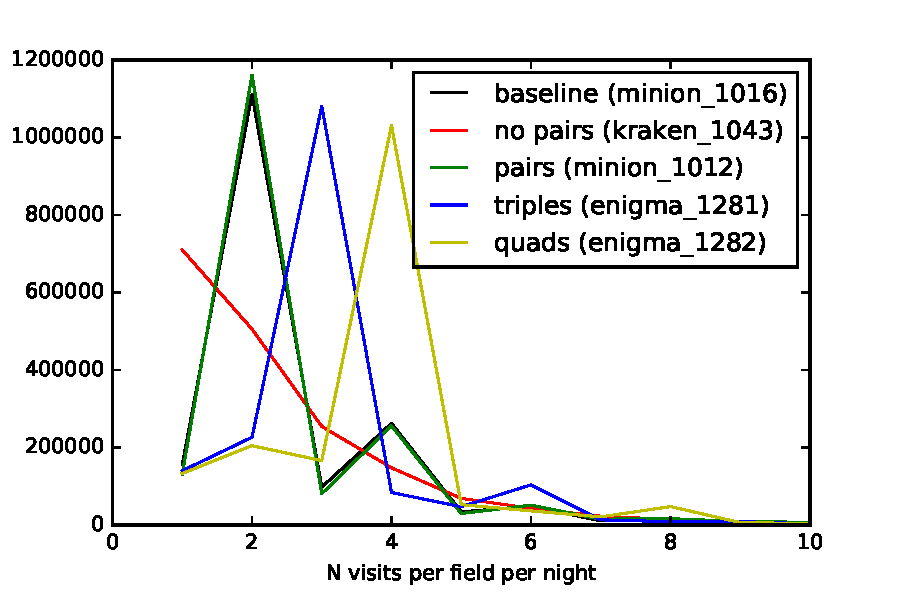
\includegraphics[angle=0,width=0.99\hsize,clip]{figs/ptq/NvisitStats.pdf}
\vskip -0.2in
\caption{The distribution of the number of visits used for nightly sequences of
length given on the horizontal axis. Only $griz$ bands are used. Note that even
``no pairs'' simulation (\opsimdbref{db:NoVisitPairs})
includes multiple visits. The highest peak is at the
requested number of visits in a sequence.}
\label{fig:NvisitStats}
\end{figure}
%%%%%%%%%%%%%%%%%%%%%%%%%%%

%%%%%%%%%%%%%%%%%%%%%%%%%%%
\begin{figure}[t!]
\vskip -1.2in
\includegraphics[angle=0,width=0.49\hsize:,clip]{figs/medintranight1.pdf}
\includegraphics[angle=0,width=0.49\hsize:,clip]{figs/medintranight2.pdf}
\vskip -1.3in
\caption{%
The comparison of the median intra-night gap (per field) distributions for the
Baseline Cadence (left)
and simulation \opsimdbref{db:NoVisitPairs}, which did not request pairs of visits per night.
Despite no need for pairs, simulation \opsimdbref{db:NoVisitPairs} produced them ``spontaneously'',
as well as longer sequences (see \autoref{fig:NvisitStats}). The mean field revisit
time is much shorter (about 6 minutes, see the right panel) than for the Baseline Cadence
(22 minutes).}
\label{fig:intranightgapCompare}
\end{figure}
%%%%%%%%%%%%%%%%%%%%%%%%%%%


\begin{figure}[h]
%\vskip -2.5in
\includegraphics[angle=0,width=0.99\hsize:,clip]{figs/med-internight.pdf}
%\vskip -2.7in
\caption{
Comparison of the median inter-night gap distribution for
\opsimdbref{db:baseCadence}, \opsimdbref{db:NoVisitPairs},
\opsimdbref{db:NEOswithVisitTriplets}, and
\opsimdbref{db:NEOwithVisitQuads}.
The peak median inter-night revisit rate (per field) is about 3 days for the
baseline cadence, \opsimdbref{db:baseCadence}, about 2 days for
\opsimdbref{db:NoVisitPairs}, and closer to 4 for both
\opsimdbref{db:NEOswithVisitTriplets} and
\opsimdbref{db:NEOwithVisitQuads}.}
\label{fig:internightgapCompare}
\end{figure}

{\bf Conclusions:}
The effect of requesting pairs, single visits, triplets or quads, is
softened with the current behavior of the scheduler, where it is not
uncommon to receive more than the requested number of visits within a
night. The inter-night revisit rates are affected, increasing the
inter-night revisit rate by about a night for triplets and quads and
reducing the inter-night revisit rate by about a night when no visit
pairs are requested (from a baseline value of about 3 nights).



% - - - - - - - - - - - - - - - - - - - - - - - - - - - - - - - - - -

%%%%%%%%%%%%%%%%%%%%%%%%%%%%%%%%%%%%%%%%%%%
\opsimdb[db:ShortExptime]{kraken\_1052}{Baseline Cadence, but with 33\% shorter exposure time.}
%%%%%%%%%%%%%%%%%%%%%%%%%%%%%%%%%%%%%%%%%%%

{\bf Motivation and description:} The optimal exposure time per visit
for the main survey, in the limit of a single value for all bands and
at all times, is in the range of about 20--60 seconds \citep[see Section
2.2.2 in the version 3.1 LSST overview paper]{IvezicEtal2008}. This
simulation investigates the effect of decreasing the exposure time per
visit to 20 seconds (from its nominal value of 30 seconds). The
shorter exposure time results in 0.22 mag shallower faint limit per
visit (the effect is larger in the $u$ band, see
\opsimdbref{db:DoubleUbandExptime}). \\

{\bf Expectations:} The total number of visits is expected to increase
by about 50\%, compared to \opsimdbref{db:baseCadence}, to 3.70 million,
for the same survey efficiency. However, the shorter exposure time
will have a significant impact on the survey efficiency: assuming a
slew time of 7 sec, the efficiency drops from 73\% to 65\% (comparing
30/(30+4+7) vs. 20/(20+4+7)). Therefore, the expected increase in the
number of visits is about 32\% and the expected number of visits is
3.2 million.  \\

{\bf Analysis Results:}  This simulated cadence is named
\opsimdbref{db:ShortExptime}. Compared to the Baseline Cadence:
\begin{enumerate}
\item The total number of visits is 3.23 million, representing an
increase of 31\% that is very close to the expected value of 32\%.
\item The median number of visits per night is 1079, or about 32\%
more than for the Baseline Cadence. The total open shutter time is 14\%
smaller for this simulation, and easily understood as due to expected
11\% decrease due to smaller surveying efficiency (the mean slew time
is the same as in the Baseline Cadence, 6.9 sec).
% 2.8 vs 2.1
\item The main survey (WFD, 18,000 sq.deg.) fields received 33\% more
visits than in the Baseline Cadence. The increase in the minimum number of
visits over that area is 9\% (from 886 to 963). In addition, another
1,000 sq.deg. (6\% of the nominal WFD) area has more than 961 visits.
\item Most other performance parameters are essentially unchanged: the
fraction of visits spent on the main survey (88\% vs. 85\%), the
median seeing in the $r$ band (0.93 arcsec vs. 0.94 arcsec), and the
median airmass (1.23 vs. 1.22).
\end{enumerate}

{\bf Conclusions:}
The comparison of \opsimdbref{db:ShortExptime} and
\opsimdbref{db:baseCadence} simulations demonstrates that the effect of
shorter exposures can be easily understood using simple efficiency
estimates. With the visit exposure time is decreased from 30 sec to 20
sec, the surveying efficiency and the total open shutter time drops by
$\sim$10\%, while the number of (shorter exposure time) visits (for
all proposals) increases by 32\%.



% - - - - - - - - - - - - - - - - - - - - - - - - - - - - - - - - - -

%%%%%%%%%%%%%%%%%%%%%%%%%%%%%%%%%%%%%%%%%%%
\opsimdb[db:LongExptime]{kraken\_1053}{Baseline Cadence, but 100\% longer exposure time.}
%%%%%%%%%%%%%%%%%%%%%%%%%%%%%%%%%%%%%%%%%%%

{\bf Motivation and description:} This simulation investigates the
effect of increasing the exposure time per visit to 60 seconds (from
its nominal value of 30 seconds). The longer exposure time results in
0.38 mag deeper faint limit per visit (the effect is larger in the
$u$ band, see \opsimdbref{db:DoubleUbandExptime}). The number of exposures per visit was kept at 2. \\

{\bf Expectations:} The total number of visits is expected to decrease by about
a factor of 2 in case of no significant impact on the survey efficiency.
However, the longer exposure time improves efficiency by a factor of
$2\times(34+7)/(64+7)-1=15\%$, and thus the expected total number of visits is
$0.5\times1.15 = 58\%$ of the number of visits in the Baseline Cadence (assuming
the same mean slew time of 7 seconds).

{\bf Analysis Results:} This simulated cadence is named \opsimdbref{db:LongExptime}.
Compared to the Baseline Cadence:
\begin{enumerate}
\item The total number of visits is 1.42 million or 58\% of the visits
obtained with the Baseline Cadence, and the total open-shutter time is
16\% higher than for the Baseline Cadence. Both results are in good
agreement with above expectations.
\item The median number of visits per night is 467, or 57\% of the
value obtained with the Baseline Cadence. The mean slew time is 0.5 sec
longer than that obtained with the Baseline Cadence.
\item This simulation has significantly different time allocation per
proposal, compared to the Baseline Cadence: 74\% spent on the WFD
proposal (vs. 85\%) and 11\%  spent on the North Ecliptic Spur proposal
(vs. 6\%)  (with smaller and less important differences for other
proposals). Because of these differences, {\it the results of this
test may not be very robust.}
\end{enumerate}

{\bf Conclusions:}
Simple estimates of the total number of visits and the
improvement in efficiency are in good agreement with delivered values. Of
course, the increased efficiency comes at the cost of fewer visits, which is
disadvantageous for time-domain science. There are other consequence of a longer
exposure time, including saturation at fainter mags, worse bleed trails and
scattered light from bright stars, and more trailing of fast-moving asteroids.

%{\bf Note to OpSim team: this simulation should be repeated} with the
%requested number of visits per field set to 60\% of the values used
%for Baseline Cadence for {\bf all} proposals. For example, instead of
%(75, 105, 240, 240, 210, 210) for Universal-18-0824B proposal, (45,
%63, 144, 144, 126, 126) should be used.  This way the additional
%observing time due to improved surveying efficiency will be allocated
%to all proposals, including WFD Cadence. {\it This simulation
%will be repeated with the same North Ecliptic Spur proposal as used
%for \opsimdbref{db:baseCadence}, and with the modified requested number of
%visits.}


% - - - - - - - - - - - - - - - - - - - - - - - - - - - - - - - - - -

%%%%%%%%%%%%%%%%%%%%%%%%%%%%%%%%%%%%%%%%%%%
\opsimdb[db:DoubleUbandExptime]{kraken\_1059}{Baseline Cadence, but with
doubled $u$-band exposure time and the number of visits halved.}
%%%%%%%%%%%%%%%%%%%%%%%%%%%%%%%%%%%%%%%%%%%

{\bf Motivation and description:} The read-out noise in the $u$ band is
not negligible compared to the background noise as in other bands, due
to darker $u$ band sky. The current best estimates for survey
performance \citep[see Table 2 in the version 3.1 LSST overview paper]{IvezicEtal2008} indicate that the {\it coadded} depth in the $u$ band
could be improved by 0.24 mag by increasing the exposure time per
visit from 30 seconds to 60 seconds
%\footnote{In the background-limited
%case, a factor of two increase of the exposure time results in 0.38
%mag deeper data. Since in the $u$ band the read-out noise is not
%negligible compared to the background noise, the total noise increases
%by less than a factor of $\sqrt{2}$ and there is an extra depth
%improvement of 0.24 mag (see eq.~7 and Table 2 the overview paper).
%Conversely, when exposure time is shorter than 30 seconds, there is an
%extra penalty of 0.16 mag, in addition to a loss of depth of 0.22 mag
%due to shorter exposure time in the limit of negligible read-out
%noise.}
(assuming the same total exposure time, which implies a
decrease in the number of visits by a factor of two). To keep the
total exposure time in the $u$ band unchanged, the requested number of
visits in this simulation is decreased by a factor of 2 relative to the
Baseline Cadence specification. \\

{\bf Expectations:} The {\it total} exposure time in the $u$ band should
remain unchanged. The single visits depth should be 0.62 mag deeper
due to increased exposure time, and the coadded depth should be 
0.24 mag deeper (due to decreased impact of readout noise). \\

{\bf Analysis Results:} This simulated cadence is named \opsimdbref{db:DoubleUbandExptime}.  Compared
to the Baseline Cadence (\opsimdbref{db:baseCadence}):
\begin{enumerate}
\item The total number of visits is 2.32 million or 95\% of the
Baseline Cadence values. The fraction of time allocated to the main
survey is 84\% vs. 85\% for the Baseline Cadence, and for the NES
proposal 7\% vs. 6\%. %Given that the NE spur proposal was different
%than for \opsimdbref{db:baseCadence}, this simulation needs to be rerun.
\end{enumerate}

{\bf Conclusions:} The $u$ band exposure time can be increased from 30
seconds to 60 seconds without a significant impact on the survey
efficiency. This change would result in a gain of about 0.2 mag in the
coadded depth, with the same total exposure time allocated to the $u$ band. 
However, the number of visits in the $u$ band would be decreased by about 
a factor of two, with a negative impact on time-domain science.
% - - - - - - - - - - - - - - - - - - - - - - - - - - - - - - - - - -

%%%%%%%%%%%%%%%%%%%%%%%%%%%%%%%%%%%%%%%%%%%
% The simulation previously known as DoubleUbandExptimewithNESpur:
\opsimdb[db:DoubleUbandExptimeSameVisits]{kraken\_1045}{Baseline Cadence, but with
doubled $u$-band exposure time and the same number of visits.}
%%%%%%%%%%%%%%%%%%%%%%%%%%%%%%%%%%%%%%%%%%%

{\bf Motivation and description:} This simulation is similar to
\opsimdbref{db:DoubleUbandExptime}, which increased the exposure time
per visit in the $u$ band from 30 seconds to 60 seconds, with the
requested number of visits decreased by a factor of 2. That change
resulted in a gain of about 0.2 mag in the coadded depth, just from reducing overheads. 
However, in order to keep the same total exposure time allocated to the $u$ band,
the number of $u$ band visits in \opsimdbref{db:DoubleUbandExptime} was
decreased by about a factor of two relative to Baseline Cadence, and this had a negative impact on
time-domain science. To further investigate this tradeoff, the \opsimdbref{db:DoubleUbandExptimeSameVisits} simulation was designed and carried out. \opsimdbref{db:DoubleUbandExptimeSameVisits} retains the Baseline Cadence
requested number of visits per field: hence, the coadded depth in the
$u$ band in this simulation could be improved by up to 0.6 mag. \\

{\bf Expectations:}  Given that about 7\% of all visits are allocated
to the $u$ band (56 out of 825), the total number of visits for other bands
will decrease when the number of the $u$ band is doubled, resulting in 
about 0.04 mag shallower data in bands other than the $u$ band. \\

{\bf Analysis Results:}  This simulated cadence is named
\opsimdbref{db:DoubleUbandExptimeSameVisits}.  Compared to the Baseline
Cadence (\opsimdbref{db:baseCadence}):
\begin{enumerate}
\item The total number of visits is 2.36 million or 95.5\% of the
Baseline Cadence values. The fraction of time allocated to the main
survey is 85\% vs. 85\% for the Baseline Cadence, and for the NES
proposal 7\% vs. 6\%.

The median number of visits in the $grizy$ filters in the main survey
decreases by about 7\%.  The median single visit depth for main survey 
is 0.53 mags deeper, and the median coadded $u$ band image is 0.50 mags 
deeper. The other filters reach shallower coadded depth 
than in the Baseline Cadence by about 0.05 mag.
\end{enumerate}


{\bf Conclusions:} When the $u$ band exposure time is increased from
30 seconds to 60 seconds, and the number of visits is kept unchanged,
the single-visit and coadded depths would be improved by about 0.5 mag. 
This improvement would come at the expense of about 7\% fewer visits in
other bands (with about 0.05 mag shallower coadded depths). These
promising results should be considered when designing the next
incarnation of baseline cadence.

% - - - - - - - - - - - - - - - - - - - - - - - - - - - - - - - - - -

%%%%%%%%%%%%%%%%%%%%%%%%%%%%%%%%%%%%%%%%%%%
\opsimdb[db:UConlyRelaxedAirmass]{minion\_1022}{Only Wide, Fast, Deep Cadence, with relaxed airmass limit.}
%%%%%%%%%%%%%%%%%%%%%%%%%%%%%%%%%%%%%%%%%%%

{\bf Motivation and description:}  What is the effect of changing the
airmass limit from 1.5 to 2.0?  To avoid complicated analysis, we use
only the WFD cadence proposal and thus compare to
\opsimdbref{db:opstwo} (which has the same footprint on ths sky).


{\bf Analysis Results:}  This simulated cadence is named
\opsimdbref{db:UConlyRelaxedAirmass}.  Compared to
\opsimdbref{db:opstwo}, it collected 99.1\% visits. This fraction is
identical to the loss of efficiency due to slightly longer mean slew
time: 7.2 sec vs. 6.8 sec. In addition,
\opsimdbref{db:UConlyRelaxedAirmass} has much worse airmass
distributions than \opsimdbref{db:opstwo}, extending to the allowed
maximum of 2.0. For example, the median for the $r$ band and WFD fields
is 1.30, compared to 1.19 for \opsimdbref{db:opstwo}.

{\bf Conclusions:} This simulation confirms that it's a bad idea to
relax the airmass limit: as a result, the airmass distribution always
widens. In addition, relaxed airmass limit tends to result in a longer
mean slew time.  For a given proposal, the airmass limit has to be as
tight as possible, while still allowing observations of all requested
fields.


% - - - - - - - - - - - - - - - - - - - - - - - - - - - - - - - - - -

%%%%%%%%%%%%%%%%%%%%%%%%%%%%%%%%%%%%%%%%%%%%%%%
\opsimdb[db:UConlyStringentAirmass]{minion\_1017}{Only Wide, Fast, Deep Cadence, with stringent airmass limit.}
%%%%%%%%%%%%%%%%%%%%%%%%%%%%%%%%%%%%%%%%%%%%%%%

{\bf Motivation and description:} What is the effect of changing the airmass
limit from 1.5 to 1.3? To avoid complicated analysis, we use only the WFD
Cadence proposal and thus compare to \opsimdbref{db:opstwo} (i.e., we are not
including the North Ecliptic Spur, South Celestial Pole, or Deep Drilling Fields
in this simulation).

 {\bf Analysis Results:}  This simulated cadence is named
 \opsimdbref{db:UConlyStringentAirmass}. Compared to
 \opsimdbref{db:opstwo}, it collected essentially the same number of
 visits. The mean slew time is also essentially unchanged (7.4 sec vs.
 7.2 sec). The airmass distributions is improved compared to
 \opsimdbref{db:opstwo}. For example, the median for the $r$ band and
 WFD fields is 1.11, compared to 1.18 for \opsimdbref{db:opstwo}.  The
 limiting coadded depth in $u$ and $g$ bands is about 0.1 mag deeper than
 for the Baseline Cadence.

{\bf Conclusions:}  It is possible to achieve the same surveying
efficiency with much more stringent airmass limit than 1.5, which was
used in most simulations to date.  {\it Given this encouraging
behavior, an analogous experiment should be executed for the Baseline
Cadence (i.e.\ a simulation like \opsimdbref{db:baseCadence}, with airmass
limit for the main survey set to 1.3) -- after the ``Western bias'' is
fixed in \OpSim version 4.}


% - - - - - - - - - - - - - - - - - - - - - - - - - - - - - - - - - -

%%%%%%%%%%%%%%%%%%%%%%%%%%%%%%%%%%%%%%%%%%%%%%%
\opsimdb[db:NormalGalacticPlane]{astro\_lsst\_01\_1004}{Extend Wide, Fast, Deep
  Cadence to the Galactic Plane.}
%%%%%%%%%%%%%%%%%%%%%%%%%%%%%%%%%%%%%%%%%%%%%%%

{\bf Motivation and description:} What is the effect of extending the
`normal' WFD Cadence and number of exposures to the region of the
Galactic Plane within the WFD declination limits?  Fields which were
previously contained in the Galactic Plane proposal, but which fell
within the range of the WFD declination limits, were reassigned to the
standard WFD proposal instead of the much more limited Galactic Plane
proposal. The remaining proposals were unchanged, and thus we compare
this to the Baseline Cadence, \opsimdbref{db:baseCadence}.

 {\bf Analysis Results:}  This simulated cadence is named
 \opsimdbref{db:NormalGalacticPlane}. Compared with
 \opsimdbref{db:baseCadence}, there are small to no changes in
 proposals other than the WFD and Galactic Plane proposals
 themselves. The fields which remained in the Galactic Plane proposal
 obtained the same number of visits as expected (30 in each
 bandpass). There were differences observed in the overall status of
 observations taken under the WFD Cadence, in the WFD proposal,
 however. The number of fields included in the WFD proposal increased
 from 2293 to 2470 ($\sim8\%$), as 177 fields were moved from the Galactic Plane
 proposal into the WFD. The total number of observations obtained by
 the WFD proposal increased from 2085270 to 2116203; an increase of
 only $1.5\%$. As a result, the median number of visits per field was
 reduced in all bands, as well as the corresponding coadded depth.

{\bf Conclusions:} In both of these runs, the WFD proposal received
about 85\% of the total number of visits in the survey. Extending the
WFD Cadence to the Galactic Plane, without increasing the
overall priority of the WFD proposal, results in slightly fewer
visits per field as a result, by about 5\%, and a slightly lower
coadded depth, by about 0.04 magnitudes. It is worthwhile to note that
increasing the priority of the WFD proposal could increase the total
fraction of time devoted to WFD, returning the typical number of
visits and coadded depth to baseline levels while decreasing time
spent in other proposals. Metrics targeted for specific science cases,
explored in later chapters, will help determine whether this is a
worthwhile trade.

\navigationbar


% --------------------------------------------------------------------

% ====================================================================
%+
% NAME:
%    rollingcadence.tex
%
% CHAPTER:
%    cadexp2.tex
%
% ELEVATOR PITCH:
%
% AUTHORS:
%    Steve Ridgway (@StephenRidgway)
%-
% ====================================================================

\section{Future Work: Rolling Cadence}
\def\secname{rolling}\label{sec:\secname}

\credit{StephenRidgway}

With a total of $\sim 800$ visits spaced approximately uniformly over 10
years, and distributed among 6 filters, it is not clear that LSST can
offer the sufficiently dense sampling in time for study of transients
with typical durations less than or $\simeq 1$week. This is particularly
a concern for key science requiring well-sampled SNIa light curves.
``Rolling'' cadences stand out as a general solution that can
potentially enhance sampling rates by 2$\times$ or more, on some of the
sky all of the time and all of the sky some of the time, while
maintaining a sufficient uniformity for survey objectives that require
it. In this section we provide an introduction to the concept of rolling
cadence, and give some examples of ways in which it can be implemented.
% We also present three preliminary \OpSim experiments, that serve to
% illustrate some of the features and challenges of the rolling cadence
% strategy.

% --------------------------------------------------------------------

\subsection{The Uniform Cadence}

Current schedule simulations allocate visits as pairs separated by 30-60
minutes, for the purposes of identifying asteroids.  For most science
purposes, the 30-60 minute spacing is too small to reveal temporal
information, and a pair will constitute effectively a single epoch of
measurement.  If the expected 824 (design value) LSST visits are
realized as 412 pairs, and distributed uniformly over 10 observing
seasons of 6 months each, the typical separation between epochs will be
4 days.   The most numerous visits will be in the $r$ and $i$
filters, and the repeat visit rate in either of these will be $\simeq$
20 days.

The possibility is still open that, for asteroid identification, visits
might be required as triples or quadrupoles, in which case the universal
temporal sampling will be further slowed by 1.5 or 2$\times$.

Under a strict universal cadence it is not possible to satisfy a need
for more frequent sample epochs.  This has led the LSST Project
simulations group to investigate the options opened up by reinterpreting
the concept of a universal cadence.  Instead of aiming for a strategy
which attempts to observe all fields ``equally'' all the time, it would
allow significant deviations from equal coverage during the survey,
returning to balance at the end of the survey.

Stronger divergence from a universal cadence, allowing significant
inhomogeneities to remain at the end of the survey, is of course
possible, but is not under investigation or discussed here.

There is currently considerable interest in the community in strategies
that provide enhanced sampling over a selected area of the sky, and
rotating the selected area in order to exercise enhanced sampling over
all of the survey area part of the time.  The class of cadences that
provides such intervals of enhanced visits, with the focus region
shifting from time to time, is termed here a ``rolling cadence.''  As a
point of terminology, observing a single sky area with enhanced cadence
for a period of time will be described as a ``roll''.

% --------------------------------------------------------------------

\subsection{Rolling Cadence Basics}

Assume a fixed number of observing epochs for each point on the sky,
nominally distributed uniformly over the survey duration.  A subset of
these can be reallocated to provide improved sampling of a sky region.
This will have the inevitable effects of: (1) reducing the number of
epochs available for that sky region during the rest of the survey, and
(2) displace observations of other sky regions during the time of the
improved temporal sampling.  In short, the cadence outside the enhanced
interval will be degraded.

The essential parameters of rolling cadence are: (1) the number of
samples taken from the uniform cadence, and (2) the enhancement factor
for the observing rate.
\href{https://project.lsst.org/meetings/ocw/sites/lsst.org.meetings.ocw/files/OpSim%20Rolling%20Cadence%20Stratgey-ver1.3.pdf}{LSST document 16370},
``A Rolling Cadence Strategy for the Operations Simulator'', by K. Cook
and S. Ridgway, contains more detailed discussion and analysis.

% --------------------------------------------------------------------
%
% \subsection{Some Example Rolling Cadence \OpSim Runs}
%
% In this section we present a set of three experimental ``Swiss Cheese''
% rolling cadence strategies, and a uniform strategy for use as a control.
%
% %%%%%%%%%%%%%%%%%%%%%%%%%%%%%%%%%%%%%%%%%%%%%%
% \opsimdb[db:SwissCheeseRollingCadence1]{ops2\_1102}{``Swiss Cheese'' rolling cadence, version 1.}
% %%%%%%%%%%%%%%%%%%%%%%%%%%%%%%%%%%%%%%%%%%%%%%%
%
% % {\bf Motivation and description:}
%
%
% %%%%%%%%%%%%%%%%%%%%%%%%%%%%%%%%%%%%%%%%%%%%%%
% \opsimdb[db:SwissCheeseRollingCadence2]{enigma\_1260}{``Swiss Cheese'' rolling cadence, version 2.}
% %%%%%%%%%%%%%%%%%%%%%%%%%%%%%%%%%%%%%%%%%%%%%%%
%
% % {\bf Motivation and description:}
%
%
% %%%%%%%%%%%%%%%%%%%%%%%%%%%%%%%%%%%%%%%%%%%%%%
% \opsimdb[db:SwissCheeseRollingCadence3]{enigma\_1261}{``Swiss Cheese'' rolling cadence, version 3.}
% %%%%%%%%%%%%%%%%%%%%%%%%%%%%%%%%%%%%%%%%%%%%%%%
%
% % {\bf Motivation and description:}
%
%
% %%%%%%%%%%%%%%%%%%%%%%%%%%%%%%%%%%%%%%%%%%%%%%
% \opsimdb[db:RollingCadenceControl]{ops2\_1098}{``Control'' simulation for comparison with the ``Swiss Cheese'' experimental rolling cadence simulations}
% %%%%%%%%%%%%%%%%%%%%%%%%%%%%%%%%%%%%%%%%%%%%%%%
%
% % {\bf Motivation and description:}
%
%
%
% % % - - - - - - - - - - - - - - - - - - - - - - - - - - - - - - - - - - -
%
% \autoref{fig:rollingcadence} illustrates the difference in how survey
% depth (characterized by the number of visits) builds up between uniform
% cadence (\opsimdbref{db:RollingCadenceControl}) and rolling cadence
% (\opsimdbref{db:SwissCheeseRollingCadence2}) strategies.
%
% \begin{figure}
%   \includegraphics[width=2.3in]{figs/ops2_1098_Count_expMJD_r_and_night_lt_365_HEAL_SkyMap.pdf}\includegraphics[width=2.3in]{figs/ops2_1098_Count_expMJD_r_and_night_lt_730_HEAL_SkyMap.pdf}\includegraphics[width=2.3in]{figs/ops2_1098_Count_expMJD_r_and_night_lt_3653_HEAL_SkyMap.pdf} \\
%   \includegraphics[width=2.3in]{figs/enigma_1260_Count_expMJD_r_and_night_lt_365_HEAL_SkyMap.pdf}\includegraphics[width=2.3in]{figs/enigma_1260_Count_expMJD_r_and_night_lt_730_HEAL_SkyMap.pdf}\includegraphics[width=2.3in]{figs/enigma_1260_Count_expMJD_r_and_night_lt_3653_HEAL_SkyMap.pdf}
%   \caption{Example of a regular uniform survey
%   (\opsimdbref{db:RollingCadenceControl}, top row) and a rolling
%   cadence survey (\opsimdbref{db:SwissCheeseRollingCadence2}, bottom row)
%   after 1, 2, and 10 years in the $r$ filter.
%   For the regular survey, the number of visits for any part of the sky
%   is relatively constant throughout the survey.  For the rolling cadence
%   simulation, there are regions with many more exposures in year one
%   which then fade in year two as other parts of the sky are
%   emphasized.}
%   \label{fig:rollingcadence}
% \end{figure}
%
%
% --------------------------------------------------------------------

\subsection{Supernovae and Rolling Cadence}
\label{sec:rolling:supernovae}

% Supernovae as a science topic are addressed elsewhere.
% In this section, the demands of SN are used to directly constrain or
% orient the rolling cadence development.

Pending more quantitative guidance, the SN objective for rolling cadence
is to obtain multi-band time series that are significantly longer than
the typical SN duration, and that have a cadence significantly faster
than uniform. As an example we discuss the option of a rolling cadence
with the regular distribution of filters.

As a simple example, consider improving the cadence by a factor of 2 or
3.  If we accept that some regions of the sky will be enhanced every
year, and that uniform sky coverage will only arrive at the end of 10
years, then we could use, e.g., 10\% of the total epochs in a single
roll.  If the enhancement is 2$\times$, each roll would last for
$\simeq$ 6 months, with high efficiency for capture of complete SN
events.  If the enhancement is 4$\times$, each roll would last for 2
months, with lower efficiency.

If it is important to achieve survey uniformity after 3 years, the
available visits for each roll would be reduced also.  With a 2$\times$
enhancement of epoch frequency, a roll would last 2 months.

Some leverage would be gained by using more than 10\% of the available
visits for a single roll.  However, this begins to impact the sampling
of slow variables reduce schedule flexibility and robustness, and should
be approached with caution.

From these examples, it appears that a 2$\times$ enhancement with
uniformity closure after 10 years is relatively feasible and promising.
Much higher gains, or more rapid closure, require additional
compromises.

% --------------------------------------------------------------------

\subsection{Fast Transients and Rolling Cadence}
\label{sec:rolling:transients}

Fast transients as a science topic are addressed elsewhere. In this
section, the demands of fast transients are used to directly constrain
or orient the rolling cadence development.

By ``fast transients'', we are referring to events that are sufficiently
fast that they are not addressed by the rolling cadence designed for SN
observations, and slow enough that they are not covered in ``deep
drilling'' type mini-surveys.  For higher tempo rolls, it is quite
difficult to obtain full color data, because of the constraints on
filter selection.  For this example, we will examine a rolling cadence
utilizing only the {\it r} and {\it i} filters, as they are used for
most visits. They are close in wavelength, and we assume that sufficient
color information will be obtained by the ``background'' uniform survey
that continues during a roll.

Again using 10\% of the available visits from the full 10 year survey
for a single roll, we find that there would be enough epochs for each
roll to acquire 1 visit per day for 21 consecutive days, giving an
enhancement of 10$\times$.

Alternatively, the same epochs could be used to observe a target every
20 minutes for 12 hours during a single night (here it is assumed that
visit pairs are not required, doubling the available epochs) for an
enhancement of 300$\times$.

Several different possible redeployments of portions of a uniform survey
have been described, each using 10\% of available time.  Of course it is
possible in principal to implement multiple options, sequentially or
maybe in parallel in some cases. This may pose considerable challenges
to the scheduling strategy design by introducing incompatible boundary
conditions.

While rolling cadences are powerful, they have limitations.  For
example, sampling events that last longer than $\simeq$1 day and less
than $\simeq$ 1 week have the obvious problem of diurnal availability.
In this example, intermediate cadences could be implemented in the
circumpolar region, where diurnal access is much extended.  This is an
example of a case in which a mini-survey of a limited number of regions
could be considered as an alternative to a rolling cadence applied to
the entire main survey.


% --------------------------------------------------------------------

\subsection{Constraints, Trades and Compromises for Rolling Cadences}
\label{sec:rolling:trades}

While rolling cadences offer some attractive benefits, it is important
to realize that rolling cadences are very highly constrained, and that
they do bring disadvantages and compromises.

There are strong arguments against beginning a rolling cadence in the
first, or even the second year of the survey.  Early in the survey, it
is important to obtain for each field/filter combination, an adequate
number of good quality photometric images, and at least one image in
excellent seeing, to support closure of photometry reductions and to
support generation of template images.

Since major science goals require a significant degree of survey
homogeneity, it may be advisable to implement a strategy that brings the
survey to nominal uniform depth at several times, e.g.\ after 3 or 5
years.  This would strongly constrain rolling cadences.

Some science objectives favor certain distributions of visits.  For
astrometry, visits early and late in the survey and at large parallax
factors, are beneficial.  Slow variables may benefit from uniform
spacing.  Rolling cadences might impact these constraints either
favorably or unfavorably.

Many objectives are served by randomization of observing conditions for
each field.  Some rolling cadences could tend to reduce this
randomization, for example by acquiring a large number of observations
during a meteorologically favorable or unfavorable season, or during a
period of instrument performance variance.

Dithering does not work gracefully with a rolling cadence, reducing
temporal coverage at the boundaries of the selected sky region.  This is
negligible for small dithers, but important for large dithers, which are
under consideration.

These cautions illustrate that evaluation of rolling cadences must be
based on the full range of schedule performance metrics, and not just
those targeted by rolling cadence development.


% --------------------------------------------------------------------

\subsection{Directions}
\label{sec:rolling:directions}

While preliminary experiments with rolling cadences have been carried
out with \OpSim, these experiments have significant deficiencies, and
are not suited for in-depth study as of this writing. Designing and 
simulating a family of rolling cadences is one of the main goals for the 
Project's ``SOCS and Scheduler'' team for the remainder of 2017. 
% However, analysis of the cadences described above may guide
% development of objectives for enhancement by rolling cadence.

Rolling cadences will be required to pass the same metrics as for other
cadences, and general requirements such as sky area, depth and visit
count must be met.  Of particular interest will be metrics that clearly
distinguish the gains available with rolling cadences -- that is,
metrics that measure schedule performance for variable targets, and
especially those with strong sampling requirements, or more rapid
variability.

% \subsubsection{Future Rolling Cadence Metrics}
%
% The following metrics, based on similar metrics developed for particular
% science objectives, may be useful in tuning rolling cadence performance:
%
% \begin{itemize}
%
% \item Observation Pairs histograms.  Visit pairs are simple and easy to
% quantify.  A pair of visits in the same filter describe a brightness
% change and constrain the rate of change. A visit pair in different
% filters (probably not coeval) constrain a color.  These metrics will
% describe how rapidly LSST can detect a change in the source fluxes. They
% will be useful for such science as early discovery of SNe, and
% identification of interesting galactic microlensing events.
%
% \item Observation Triplets histograms. Similar to Pairs, but with
% closely spaced triplets allowing detection and confirmation of transient
% events \citep[as described by][]{LundEtal2016}.
%
% \item Period determination metric.  Compute a measure of the period
% determination accuracy after a given time interval, as a function of
% period. A complete analysis would allow use of real light curves for
% various object types with realistic brightness distributions.  A simpler
% approach would use a single example light curve and a fixed measurement
% error value. A simplest approach would be based on the sampling function
% and its power spectrum \citep{LundEtal2016}.  This metric group would
% rate simulation performance for period determination of periodic
% variables - mostly stars.
%
% \item Sampling of SNe light curves.  The most complete metric would
% count the number of SNe (of various types) light curves that would be
% well sampled (according to defined criteria), based on analysis of
% realistic simulated data.  A simpler metric would be based on estimated
% sampling requirements and cadence without considering brightness. The
% latter could be used initially, pending replacement (or calibration)
% with more extensive simulations.
%
% \item Time series count. For any transient or irregular variable, the
% optimum observational data will require multiple time and color samples
% within the duration of the event. Since the category of transients may
% include discoveries, it is not possible to exhaustively specify the
% source characteristics. A time series can be defined to consist of a
% series of samples, over some total duration T, with sampling interval t
% to tolerance d. The count of time series depends on the total duration,
% the number of samples, as well as the filter selection, so the challenge
% is how to visualize this information, and how to extract useful
% characteristic summary measures of performance.  This type of data can
% be valuable for identification and study of rapid phenomena such as
% stellar flares, binary mass transfer events, and exoplanet transits, and
% for slower events such as AGN reverberation mapping.
%
% \end{itemize}

% ====================================================================

\navigationbar


% % --------------------------------------------------------------------
%
% \section{Future Work}
% \def\secname{cadexp:future}\label{sec:\secname}
%
%
% \subsection{Ongoing: Extended time-domain metrics}
%
% A number of very sophisticated time-domain metrics have been
% implemented in recent MAF development cycle (and some were contributed
% by the community) but they have not been systematically run yet on all
% available simulations. Time-domain metrics, together with metrics for
% analyzing special programs (e.g. deep drilling programs), will be
% further expanded in the next development cycle.
%
%
% \subsection{Ongoing: Rolling Cadence experiments}
%
% Analysis of a few prototype runs (\texttt{ops2\_1102},
% \texttt{enigma\_1260}, \texttt{enigma\_1261}), which implemented the
% so-called ``swiss cheese rolling cadence'' is in progress.
%
%
%
% \navigationbar
%
% % --------------------------------------------------------------------

\section{Summary}
\def\secname{cadexp:summary}\label{sec:\secname}

The most important conclusion of this chapter is that the upper limit on
possible scheduling efficiency improvements for the Baseline Cadence is
close to 6\%. This conclusion is by and large based on the fact that
the mean slew time for the Baseline Cadence is 6.9 sec, and
thus only slightly larger than the design specifications for the
system slew and settle time of 4.5 sec.  Nevertheless, there are a
number of features to understand, and some to fix, and there is
substantial optimization potential in temporal sampling functions and
further optimization of the sky area and observing strategy details,
that can result in enhanced science even with the same integrated
open-shutter time (e.g. by obtaining deeper data through an improved
sampling of observing conditions).

\vskip 0.2in
The main other questions addressed here are:

\begin{enumerate}

\item {\it By what factor could we exceed the SRD design specification
for the number of visits if only the WFD Cadence proposal was
implemented?}

A simulation that only implemented the WFD Cadence proposal exceeded
the design specification for the number of visits by about 40\% (over
the design specification for the sky area of 18,000 sq.deg.)

\item {\it By what factor could we exceed the SRD design specification
for the sky coverage if only the WFD Cadence proposal was
implemented with the design specification for the number of visits?}

The Pan-STARRS-like strategy results in about 40\% larger sky
coverage (about 25,000 sq.deg.), with the mean number of visits at
92\% of the design specification. The total number of visits is the
same as for the Baseline Cadence, implying similar surveying efficiency.

Therefore, the available ``margin'' relative to the SRD design specifications
for the main survey is equivalent to about 30-40\% larger sky coverage, or
about 30-40\% more visits per field. The SRD assumes that 10\% margin
will be available for other programs. The implied ``survey reserve'',
relative to the WFD Cadence design specifications from the SRD, can
be used to:
  \begin{enumerate}
  \item increase the number of visits per field over the WFD area,  or
  \item increase the surveyed area while keeping the number of visits
  per field statistically unchanged, or
  \item increase both area and the number of visits, and/or
  \item execute additional programs (the current baseline).
  \end{enumerate}

\item {\it What is the effect of auxiliary proposals on surveying
efficiency?}

A comparison of simulations which only implemented the WFD Cadence
proposal to those that included all other programs did not show a
significant change of efficiency (older simulations, not analyzed
here, showed increases in surveying efficiency of up to about 3\% due
to shorter slewing time).


\item {\it What is the effect of visit pairs on surveying efficiency? }

Relinquishing the visit pair requirement results in up to 2-3\%
improvement of the surveying efficiency. The impact on some
time-domain science would be positive, while for NEO and main-belt
asteroid science it would be strongly negative.


\item {\it Can the effects of variations of the visit exposure time on
surveying efficiency be predicted using simple efficiency estimates?}

Simple estimates based on comparing exposure (open shutter) and total
visit times are in good agreement with simulations. Decreasing the
visit exposure time to 20 seconds decreases the total open shutter
time by 10\%, and increasing it to 60 seconds increases the total open
shutter time by 16\%, relative to the Baseline Cadence and standard
exposure time of 30 seconds. The number of visits changes by factors
of 1.35 and 0.58.


\item {\it What are the effects of doubling the exposure time only in
the $u$ band?}

The effect of doubling the exposure time only in the $u$ band, while
simultaneously halving the number of requested visits, has no
significant effect on the survey efficiency.

The effect of doubling the exposure time only in the $u$ band, with
the number of requested visits unchanged, is a decrease in the number
of visits in other bands by about 6\%.


\item {\it What is the impact of the hard airmass limit, $X<1.5$, on the
surveying efficiency?}

It is a very bad idea to relax the airmass limit! It is possible to
achieve the same surveying efficiency with a much more stringent airmass
limit than 1.5, which was used in most simulations to date.

\end{enumerate}

% --------------------------------------------------------------------

\navigationbar

%%  LocalWords:  STARRS cadexp Bremerton MAF opsim baseCadence Aitoff
%%  LocalWords:  airmass coadded WFD Msec airmassenigma ugrizy ivezic
%%  LocalWords:  SRD coaddm urz ury parapmenigma OpSim pre HAenigma
%%  LocalWords:  AltAzenigma radians enigmaGapAll enigmaGapr SNe griz
%%  LocalWords:  enigmaMAXGapAll enigmaEarlySNe Intra opstwoPS opstwo
%%  LocalWords:  UConlyNoVisitPairs NoVisitPairs kraken ShortExptime
%%  LocalWords:  DoubleUbandExptime LongExptime UConlyRelaxedAirmass
%%  LocalWords:  DoubleUbandExptimeSameVisits UConlyStringentAirmass
%%  LocalWords:  NEO PHA NEOs PHAs MOID Neptunian detections intra eq
%%  LocalWords:  differencing NEOsNoVisitPairs NEOswithVisitPairs LMC
%%  LocalWords:  NEOswithVisitTriplets NEOwithVisitQuads NvisitStats
%%  LocalWords:  enigmaNEO intranightgapCompare NEOquads Gould's SMC
%%  LocalWords:  Stubbs multi yoachim rhiannonlynne quartiles swiss
%%  LocalWords:  strawman unrequested
